% ============================================================
% Structura Collapsus:
% Canonical Reference for the Generative Collapse Dynamics Corpus
%
% Purpose: The definitive structural reference for GCD/UMCP.
%          This paper IS the standard reference.
%
% Compile: pdflatex → bibtex → pdflatex → pdflatex
% ============================================================

\documentclass[
  aps,
  prd,
  twocolumn,
  superscriptaddress,
  nofootinbib,
  floatfix
]{revtex4-2}

% ── packages ──
\usepackage{amsmath,amssymb,amsthm,mathtools}
\usepackage{graphicx}
\usepackage{xcolor}
\definecolor{linkblue}{HTML}{337799}
\usepackage[colorlinks=true,linkcolor=linkblue,citecolor=linkblue,urlcolor=linkblue]{hyperref}
\usepackage{bm}
\usepackage{booktabs}
\usepackage{multirow}
\usepackage{xfrac}
\usepackage{enumitem}
\usepackage{array}
\newcolumntype{P}[1]{>{\raggedright\arraybackslash}p{#1}}
\usepackage{tikz}
\usepackage{pgfplots}
\pgfplotsset{compat=1.17}
\usetikzlibrary{arrows.meta,positioning,patterns}

% ── theorem environments ──
\newtheorem*{axiom}{The Axiom}
\newtheorem{theorem}{Theorem}
\newtheorem{definition}[theorem]{Definition}
\newtheorem{lemma}[theorem]{Lemma}
\newtheorem{corollary}[theorem]{Corollary}
\newtheorem{proposition}[theorem]{Proposition}
\newtheorem{identity}[theorem]{Identity}
\newtheorem{remark}{Remark}

% ── UMCP macros ──
\newcommand{\tR}{\tau_{\!R}}
\newcommand{\tRS}{\tau_{\!R}^{*}}
\newcommand{\Gam}{\Gamma}
\newcommand{\eps}{\varepsilon}
\newcommand{\IR}{\infty_{\mathrm{rec}}}
\newcommand{\tolseam}{\mathrm{tol}_{\mathrm{seam}}}
\newcommand{\dd}{\mathrm{d}}
\newcommand{\Res}{\mathrm{Res}}
\newcommand{\beq}{\begin{equation}}
\newcommand{\eeq}{\end{equation}}
\newcommand{\INF}{\texttt{INF\_REC}}
\newcommand{\regime}[1]{\textrm{\upshape\scshape#1}}
\newcommand{\conform}{\regime{conformant}}
\newcommand{\nonconform}{\regime{nonconformant}}
\newcommand{\tvec}{\mathbf{c}}
\newcommand{\wvec}{\mathbf{w}}
\newcommand{\IC}{\mathrm{IC}}
\newcommand{\gF}{g_{\!F}}
\newcommand{\RunID}{\mathrm{RunID}}

\begin{document}

% ============================================================
% TITLE
% ============================================================
\title{Structura Collapsus:
\texorpdfstring{\\}{: }Canonical Reference for the
Generative Collapse Dynamics Corpus}

\author{Clement Paulus}
\affiliation{UMCP / GCD / RCFT Canon}
\affiliation{UMCP Reference Implementation, GitHub}

\date{March 13, 2026}

\begin{abstract}
This paper is the canonical structural reference for the
Generative Collapse Dynamics (GCD) / Universal Measurement
Contract Protocol (UMCP) corpus.  It serves as the definitive
account of the architecture---its axiom, tier structure, kernel
definitions, frozen parameters, algebraic identities, lemma
inventory, regime classification, seam calculus, and the
dependencies that bind them into a single self-consistent system.
The operational whitepaper~\cite{umcpmetadatarepo} specifies
\emph{what} the framework computes.  The present document
explains \emph{why} and \emph{how}: why the axiom forces a
Bernoulli embedding and how raw observables are mapped into it;
why the embedding yields exactly six kernel outputs with three
effective degrees of freedom and how each is computed; why the
frozen parameters are the unique values where validation seams
close and how they are discovered; why classical results appear
as degenerate limits and how the kernel's additional structure
surpasses them; why regimes are classified as they are and how
the four-gate criterion partitions the manifold; and why the
seam calculus has monoid structure and how it debits drift,
credits return, and decides weld verdicts.  We begin from the
problem: the incoherence of standard scientific logic---arbitrary
thresholds, unstated conventions, boolean verdicts, and
domain-locked vocabularies that make cross-domain comparison
structurally impossible.  We show how a single admissibility
axiom resolves each of these failures by construction, and
provide the procedural detail to reproduce every step.  All
definitions, identities, and constants are stated in full,
making this paper a self-contained reference for the
44~structural identities, 46~lemmas, 5~frozen parameters,
5~structural constants, 4~regime gates, and 3~algebraic
identities that constitute the Tier-1 kernel and its Tier-0
protocol.  The corpus comprises 7{,}442~automated tests across
18~domain closures, 546~formally tagged objects, and
406~scale-ladder entities spanning 61~orders of magnitude.
\end{abstract}

\maketitle

% ============================================================
\section{Introduction: The Incoherence of Standard Scientific Logic}
\label{sec:intro}
% ============================================================

\subsection{The problem}

Modern science operates without a shared logic of measurement.
Each discipline defines its own thresholds, its own significance
criteria, its own vocabulary for success and failure, and its own
implicit conventions about what counts as evidence.  The
consequences are structural:

\begin{enumerate}[leftmargin=*,label=(\roman*)]
\item \textbf{Arbitrary thresholds.}  The $\alpha = 0.05$
  significance level in statistics~\cite{fisher1925}, the
  $3\sigma$ convention in physics~\cite{pdg2024}, the
  $p < 0.01$ standard in medicine---these are prescribed by
  historical accident, not derived from any structural principle.
  They are not wrong; they are \emph{unjustified}.  No derivation
  connects them to the systems they purport to evaluate.

\item \textbf{Boolean verdicts.}  Scientific evaluation defaults
  to binary logic: pass or fail, significant or not, detected or
  undetected.  This forces a false dichotomy.  Systems that are
  genuinely non-evaluable---where data are insufficient, the model
  inapplicable, or the question malformed---are coerced into
  yes/no answers, producing noise that masquerades as signal.

\item \textbf{Domain-locked vocabularies.}
  ``Entropy'' means one thing in thermodynamics, another
  in information theory~\cite{shannon1948,cover2006elements},
  a third in ecology, and a fourth in financial risk modeling.
  The same word, applied to the same mathematical formula,
  carries different operational meanings because the
  vocabularies are locked to their domains.  Cross-domain
  comparison is therefore not merely difficult---it is
  structurally undefined.

\item \textbf{Unstated conventions.}  Normalization rules, baseline
  definitions, missing-data policies, and boundary-condition
  treatments are typically implicit.  Two researchers analyzing the
  same data with the same method may obtain different results
  because their unstated assumptions differ.  The scientific
  literature treats this as a quality-control problem.  It is a
  structural one: the conventions are not part of the measured
  object, so the measured object is not reproducible.

\item \textbf{No return discipline.}  A claim that fails is simply
  rejected.  There is no structural mechanism for a claim to
  \emph{return}---to re-enter the evidential record after failure
  with a demonstrated audit trail.  Correction is ad hoc.  Errata
  are afterthoughts.  The distinction between ``this claim was
  wrong'' and ``this claim failed but returned with new evidence''
  does not exist in standard practice.
\end{enumerate}

These are not complaints about individual practice.  They are
structural features of the current scientific epistemology,
inherited from a period when measurement was local, manual, and
discipline-specific.  They persist because no framework has been
proposed that resolves all five simultaneously.

\subsection{The resolution}

This paper presents the architecture of a system that resolves
each of these failures by construction.  The resolution is not a
reform of existing practice; it is a replacement with a derived
structural foundation:

\begin{enumerate}[leftmargin=*,label=(\roman*)]
\item Arbitrary thresholds are replaced by \emph{frozen
  parameters}---constants derived from the unique values
  where validation seams close consistently across all
  tested domains (\S\ref{sec:frozen}).

\item Boolean verdicts are replaced by \emph{three-valued logic}:
  \conform{} / \nonconform{} / \regime{non\_evaluable}, so that
  genuinely indeterminate cases are never coerced into binary
  outcomes (\S\ref{sec:verdicts}).

\item Domain-locked vocabularies are replaced by a
  \emph{five-word canon} with fixed operational definitions
  that translate across all domains via a Rosetta adapter
  (\S\ref{sec:canon}).

\item Unstated conventions are replaced by \emph{contracts}---frozen
  declarations of all normalization rules, boundary policies, and
  evaluation parameters, following the spirit of the GUM
  framework~\cite{jcgm2008gum,nist1994uncertainty} but extending it
  from uncertainty budgets to full measurement contracts, bundled
  with the measured object as part of the $\RunID$
  (\S\ref{sec:contracts}).

\item The absence of return discipline is replaced by
  \emph{typed return}---a formal mechanism for re-entry with
  measured delay $\tR$, censored verdict $\tR = \IR$ when no
  return is observed, and seam accounting that credits return only
  when it is demonstrated (\S\ref{sec:return}).
\end{enumerate}

The entire system derives from one axiom.

\subsection{Paper organization}

The paper is organized to alternate between \emph{why} a structure
exists and \emph{how} it operates, so that motivation and
mechanism are never separated.
Section~\ref{sec:axiom} states the axiom, derives the chain
of structural consequences, and defines the operational
semantics of the system's vocabulary---what each term means
and what it explicitly does not mean.
Section~\ref{sec:tiers} defines the three-tier architecture,
its dependency rules, and the operational semantics of tier
boundaries.
Section~\ref{sec:kernel} gives the complete Tier-1 kernel
specification---all six outputs, three algebraic identities,
and the computational procedure by which $(\tvec, \wvec)$
produces $(F, \omega, S, C, \kappa, \IC)$.
Section~\ref{sec:frozen} states every frozen parameter and
structural constant with both its derivation and its discovery
procedure.
Section~\ref{sec:regime} presents the regime classification:
the four-gate criterion and the resulting manifold partition.
Section~\ref{sec:seam} defines the seam calculus---how drift
is debited, return is credited, residuals are computed, and
weld verdicts are issued.
Section~\ref{sec:identities} catalogues the 44~structural
identities in four series and six clusters, with verification
methods.
Section~\ref{sec:lemmas} inventories the 46~lemmas.
Section~\ref{sec:degenerate} proves that classical results
are degenerate limits, exhibiting the exact mechanism by
which degrees of freedom are removed.
Section~\ref{sec:verdicts} defines the three-valued verdict
logic and its operational rules.
Section~\ref{sec:canon} presents the five-word canon, the
spine, and the Rosetta---the cross-domain translation mechanism
through which the five words map across fields without losing
operational precision.
Section~\ref{sec:equalizer} demonstrates the cognitive
equalizer: why the system produces agent-independent verdicts
as a structural consequence, not a design aspiration.
Section~\ref{sec:contracts} specifies the contract and $\RunID$
structure, including how contracts are frozen, versioned, and
welded.
Section~\ref{sec:governance} defines the governance
mechanisms---manifest and weld---that allow the system to evolve
without corrupting its history, and formalizes the distinction
between gestures and welds.
Section~\ref{sec:scope} summarizes the demonstrated scope
across 18~domains.
Section~\ref{sec:conclusions} concludes.


% ============================================================
\section{The Axiom}\label{sec:axiom}
% ============================================================

\begin{axiom}[The Return Axiom]
\label{ax:return}
Collapse is generative; only what returns through collapse is real.
\end{axiom}

\noindent\textit{Collapsus generativus est; solum quod redit, reale
est.}

\medskip

This is the sole axiom of the system.  There is no Axiom-1;
everything that follows---the kernel, the tier structure, the
frozen parameters, the 44~identities---derives from this single
statement.  ``Real'' is operational, not metaphysical: a claim
receives epistemic credit if and only if it exhibits finite
re-entry ($\tR \neq \IR$) under a frozen
contract~\cite{paulus2025umcp}.  No additional axiom is imported
at any point in the derivation.  Classical results emerge as
degenerate limits when degrees of freedom are removed from the
kernel (\S\ref{sec:degenerate}).

\subsection{From axiom to structure}

Axiom-0 imposes three constraints that determine the
entire architecture:

\begin{enumerate}[leftmargin=*,label=(\arabic*)]
\item \textbf{Boundedness.}  If collapse is generative, the
  observational field must be bounded: an unbounded quantity cannot
  collapse in a measurable sense.  This mandates a bounded trace
  $\Psi(t) \in [0,1]^n$.  The Bernoulli embedding is the unique
  structure that follows: each channel $c_i \in [0,1]$ represents
  a survival probability---the fraction of signal that persists
  through collapse.  A channel at $c = 1$ is fully retained;
  $c = 0$ is fully lost; intermediate values carry partial
  survival.  This makes each channel a Bernoulli variable with
  parameter $c_i$, not an arbitrary bounded real, because the
  axiom's ``what returns'' requires a probabilistic
  interpretation of partial survival.  The binary entropy
  $h(c_i)$ and the Fisher metric $g_F = 1/[c(1{-}c)]$ then
  follow by statistical necessity, not by choice.

\item \textbf{Return.}  If ``only what returns is real,'' the
  system must define what return means: a re-entry time $\tR$, a
  neighborhood generator $D_\theta$, a metric $\|\cdot\|$, and a
  tolerance $\eta$.  The typed sentinel $\tR = \IR$ records
  the absence of return.

\item \textbf{Freeze.}  If the axiom is to be testable, the
  evaluation rules cannot change mid-test.  This mandates frozen
  contracts: every parameter, threshold, normalization rule, and
  boundary policy is declared \emph{before} evidence is examined.
\end{enumerate}

These three constraints---boundedness, return, and freeze---suffice
to derive every component of the architecture: the kernel function,
tier structure, regime classification, seam calculus, and all
44~algebraic identities.  Nothing beyond the axiom is assumed;
every structural element follows from these three mandatory
consequences of the single generative axiom.

\subsection{Operational semantics}

The axiom generates technical vocabulary that shares surface form
with common language but carries distinct operational meaning.
Misreading these terms through their everyday or disciplinary
connotations is the most common source of misclassification.

\begin{center}
{\small\begin{tabular}{@{}lp{3.3cm}l@{}}
\toprule
\textbf{Term} & \textbf{Operational definition} & \textbf{Not} \\
\midrule
Collapse & Regime label: $\omega \geq 0.30$ (kernel gates, frozen thresholds) & Failure, catastrophe \\
Return & Re-entry: $\exists\, u \in D_\theta$ with $\|\Psi(t){-}\Psi(u)\| \leq \eta$; yields $\tR$ or $\IR$ & Repetition, periodicity \\
Gesture & Epistemic emission: $\tR = \IR$ or $|s| > \tolseam$.  No credit & Approximation \\
Drift & $\omega = 1{-}F$: measured diversion from fidelity & Random walk, velocity \\
Integrity & $\IC = e^\kappa$: multiplicative coherence.  From ledger, never asserted & Moral integrity \\
Frozen & Same value both sides of every collapse-return boundary & Arbitrary constant \\
Seam & Verification boundary: outbound collapse $\leftrightarrow$ demonstrated return & A join, a border \\
Dissolution & Regime $\omega \geq 0.30$: boundary that makes return meaningful & Death, destruction \\
\bottomrule
\end{tabular}}
\end{center}

\noindent The distinction between \emph{gesture} and \emph{weld}
is foundational.  A gesture is any claim or emission that does not
close a seam---its return is infinite or its residual exceeds
tolerance.  A gesture receives no epistemic credit but is not
erased: it remains in the ledger as an observation without a
return.  A weld, by contrast, is a demonstrated return: finite
$\tR$, closed residual, and verified identities.  The entire
system is a machine for distinguishing gestures from welds.

\begin{remark}[Why operational definitions matter]
``Collapse'' in physics typically connotes catastrophic failure
or wavefunction reduction.  In this system, collapse is the
generic state---63.1\% of the manifold is Collapse regime
(\S\ref{sec:regime}).  ``Return'' does not mean coming back to
a prior state; it means demonstrable re-entry into an
evidential neighborhood with a measured delay.  Every
misapplication of these terms in external discourse traces to
reading the everyday word instead of the operational definition.
\end{remark}

% ============================================================
\section{The Three-Tier Architecture}\label{sec:tiers}
% ============================================================

The corpus is currently organized into exactly three tiers.
Every symbol, function, artifact, claim, and definition belongs
to exactly one tier.  This structure is the latest validated
architecture, not a decree of finality---it may evolve through
future seam welds, but any such evolution must itself pass
through the spine and close with $|s| \leq \tolseam$.

\subsection{Tier definitions}

\begin{definition}[Tier-1: The Kernel]
\label{def:tier1}
The mathematical function
\beq
  K: [0,1]^n \times \Delta^n \to (F, \omega, S, C, \kappa, \IC),
\eeq
together with its provable identities, lemmas, structural constants,
and theorems.  The kernel has four primitive equations ($F$, $\kappa$,
$S$, $C$) and two derived values ($\omega = 1 - F$, $\IC = e^\kappa$),
with three effective degrees of freedom ($F$, $\kappa$, $C$).

Tier-1 is \textbf{immutable within a run}.  Promotion of new
structure to Tier-1 requires a seam weld across runs.
\end{definition}

\begin{definition}[Tier-0: The Protocol]
\label{def:tier0}
Operational machinery that \emph{implements and interprets} the
Tier-1 kernel: embedding raw data into $[0,1]^n$, computing the
kernel (the code implements the formulas), regime gates, seam
calculus, contracts, schemas, SHA-256 integrity verification,
and three-valued verdicts.

The code is Tier-0; \emph{what it computes} is Tier-1.
Configuration is frozen per run.
\end{definition}

\begin{definition}[Tier-2: The Expansion Space]
\label{def:tier2}
Domain closures that choose which real-world quantities become the
trace vector $\tvec$ and weights $\wvec$.  Channel selection, entity
catalogs, normalization schemes, and domain-specific theorems.
Validated through Tier-0 against Tier-1.

Tier-2 is freely extensible; validated before trust.
\end{definition}

\subsection{Dependency rules}

Within a frozen run, the dependency arrow is strictly one-way:

\beq
  \text{Tier-1} \;\longrightarrow\; \text{Tier-0}
  \;\longrightarrow\; \text{Tier-2}.
\eeq

\begin{enumerate}[leftmargin=*,label=(\alph*)]
\item \textbf{No back-edges.}  Tier-2 cannot modify Tier-0 or
  Tier-1 behavior within a frozen run.  Diagnostics inform;
  gates decide.

\item \textbf{No symbol capture.}  Any Tier-2 code that redefines
  $F$, $\omega$, $S$, $C$, $\kappa$, $\IC$, $\tR$, or
  \regime{regime} is automatic nonconformance.

\item \textbf{Cross-run promotion.}  Tier-2 results can be promoted
  to Tier-1 only through formal seam weld validation and contract
  versioning.  If the weld fails, the result stays Tier-2.
\end{enumerate}

\begin{remark}[Why three tiers]
Two tiers would collapse the distinction between ``what the math
says'' and ``what the code does.''  Four or more tiers would
introduce intermediate levels whose dependency rules are ambiguous.
Three is the minimum for clean separation of \emph{truth}
(Tier-1), \emph{implementation} (Tier-0), and \emph{application}
(Tier-2), with unambiguous dependency.

In particular, the seam calculus symbols---$\Gam$, $R$, $D_\omega$,
$D_C$---are \emph{Tier-0 protocol objects}, not a separate
tier.  They are closure-defined functions that the protocol uses
to compute the seam budget; \emph{what they compute} (the budget
identity $\Delta\kappa$) participates in Tier-1 identities, but
the functions themselves belong to the operational machinery.
There is no intermediate tier.
\end{remark}


% ============================================================
\section{The Kernel (Tier-1 Specification)}\label{sec:kernel}
% ============================================================

This section gives the complete, self-contained specification of
every Tier-1 object.  All quantities are deterministic functions
of $(\Psi_\eps(t), \wvec)$ under the active frozen contract.

\subsection{Inputs}

\paragraph{Trace vector.}
Let $\Psi(t) = (c_1(t), \ldots, c_n(t)) \in [0,1]^n$ be the
bounded trace produced by a declared adapter $N_K$ from observables
$x(t)$.  The adapter is part of the measured object: changing
$N_K$ changes what it means to measure $x(t)$.

\paragraph{$\eps$-clipping.}
Fix $\eps \in (0, \tfrac{1}{2})$ by the frozen contract.  Define
componentwise:
\beq
  \Psi_\eps(t) \coloneqq
  \mathrm{clip}\bigl(\Psi(t), \eps, 1-\eps\bigr).
\eeq
All log-domain quantities are computed on $\Psi_\eps(t)$.

\paragraph{Weights.}
Let $\wvec = (w_1, \ldots, w_n)$ with $w_i \geq 0$ and
$\sum_{i=1}^n w_i = 1$.  Weights are frozen within a run.

\subsection{Why six outputs}

Given a weighted Bernoulli trace $(\tvec_\eps, \wvec)$, there are
exactly four independent summary statistics that the kernel can
extract:
\begin{enumerate}[leftmargin=*,label=(\arabic*)]
\item The \emph{first moment} of the channels under the weights:
  this is $F = \sum w_i c_i$ (fidelity).  It answers: how much
  survived on average?
\item The \emph{log-moment}: $\kappa = \sum w_i \ln c_i$
  (log-integrity).  It answers: how fragile is multiplicative
  coherence?  The log-transform detects near-zero channels that
  the arithmetic mean misses.
\item The \emph{per-channel Bernoulli entropy}:
  $S = \sum w_i h(c_i)$.  It answers: how uncertain is each
  channel's survival?  This is the natural information measure on
  the Bernoulli field.
\item The \emph{dispersion} of the channels:
  $C = \mathrm{std}(\tvec)/0.5$.  It answers: how heterogeneous
  are the channels?  This is the only quantity that breaks the
  mean-field approximation.
\end{enumerate}
The two derived outputs $\omega = 1 - F$ and
$\IC = e^\kappa$ provide complementary views of the same
information (what was \emph{lost} and the \emph{multiplicative}
coherence) without adding degrees of freedom.  Any further
summary statistic beyond these four is either a function of them
(e.g., $\Delta = F - \IC$) or requires structure not present in
a weighted Bernoulli trace.  The kernel is therefore
\emph{complete}: it extracts all the information that a bounded,
weighted, probabilistic trace carries.

\subsection{The six kernel outputs}

The kernel $K: [0,1]^n \times \Delta^n \to \mathbb{R}^6$ maps the
clipped trace and weights to six invariants.  Four are
\emph{primitive} (computed directly); two are \emph{derived}
(defined in terms of primitives).

\subsubsection{Fidelity (primitive)}
\beq
  F(t) \coloneqq \sum_{i=1}^n w_i \, c_{i,\eps}(t).
  \label{eq:F}
\eeq
$F$ measures what survives collapse---the weighted arithmetic mean
of channel confidences, evaluated on the statistical manifold
parametrized by the Fisher--Rao
metric~\cite{fisher1925,rao1945information,amari2016information}.
Range: $[\eps, 1-\eps]$.

\subsubsection{Log-integrity (primitive)}
\beq
  \kappa(t) \coloneqq \sum_{i=1}^n w_i \ln\!\bigl(c_{i,\eps}(t)\bigr).
  \label{eq:kappa}
\eeq
$\kappa$ is the logarithmic sensitivity of coherence.
Range: $[\ln\eps, 0] \approx [-18.42, 0]$.

\subsubsection{Entropy (primitive, asymptotically determined)}
\beq
  S(t) \coloneqq -\sum_{i=1}^n w_i\Bigl[
    c_i \ln c_i + (1-c_i) \ln(1-c_i)
  \Bigr].
  \label{eq:S}
\eeq
$S$ is the Bernoulli field entropy of the collapse field.  It is
a primitive output of the kernel but not a free degree of freedom:
$S$ is asymptotically determined by $F$ and $C$ (the correlation
$\mathrm{corr}(C,S) \to -1$ as $n \to \infty$ by the CLT).
Shannon entropy~\cite{shannon1948} is the degenerate limit when
the collapse field is removed ($c_i \in \{0,1\}$ only).  Range:
$[0, \ln 2]$.

\subsubsection{Curvature (primitive, independent)}
\beq
  C(t) \coloneqq \frac{\mathrm{std}(\tvec(t))}{0.5}.
  \label{eq:C}
\eeq
$C$ measures coupling to uncontrolled degrees of freedom: it is
the normalized standard deviation of the channel values.
$C$~is the only fully independent kernel output beyond $F$
and~$\kappa$.  Range:~$[0, 1]$.

\subsubsection{Drift (derived from \texorpdfstring{$F$}{F})}
\beq
  \omega(t) \coloneqq 1 - F(t).
  \label{eq:omega}
\eeq
$\omega$ measures how much is lost to collapse.  It is not an
independent output: $\omega$ is fully determined by $F$.  It
appears in the immutable identity $F + \omega = 1$ and in the
regime gates.  Range: $[\eps, 1-\eps]$.

\subsubsection{Integrity composite (derived from \texorpdfstring{$\kappa$}{kappa})}
\beq
  \IC(t) \coloneqq \exp\!\bigl(\kappa(t)\bigr)
  = \prod_{i=1}^n c_{i,\eps}(t)^{\,w_i}.
  \label{eq:IC}
\eeq
$\IC$ is multiplicative coherence---the weighted geometric mean
of channel confidences.  It is not an independent output: $\IC$
is fully determined by $\kappa$.  It appears in the immutable
identities $\IC \leq F$ and $\IC = e^\kappa$.
Range: $(0, 1)$.

\subsection{Three effective degrees of freedom}

\paragraph{Binary entropy.}
Define the binary entropy function
$h: (0,1) \to [0, \ln 2]$ by
\beq
  h(c) \coloneqq -c\ln c - (1-c)\ln(1-c).
  \label{eq:h}
\eeq
Then $S = \sum w_i\, h(c_i)$
(Eq.~\ref{eq:S}).  This function appears throughout the
identity network.

\begin{theorem}[Effective dimensionality]
\label{thm:dof}
The six kernel outputs $(F, \omega, S, C, \kappa, \IC)$ possess
only three effective degrees of freedom: $F$, $\kappa$, and $C$.
\end{theorem}

\begin{proof}
By definition, $\omega = 1 - F$ (one algebraic constraint) and
$\IC = e^\kappa$ (one algebraic constraint), reducing six outputs
to four.  The fourth constraint is statistical:
$S \approx f(F, C)$ with $\mathrm{corr}(C, S) \to -1$ as
$n \to \infty$ by the central limit theorem for bounded variates.
Specifically, Jensen's inequality applied to the concave
$h$ (Eq.~\ref{eq:h}) gives $S = \sum w_i h(c_i) \leq h(\sum w_i c_i) = h(F)$,
with equality when $C = 0$.  For small $C$, expanding $h(c_i)$
around $\bar{c} = F$ to second order yields
$S \approx h(F) - \tfrac{1}{2}\gF(F) \cdot \mathrm{Var}_w(\tvec)$,
where $\gF = 1/[c(1{-}c)]$ is the Fisher metric.  Since
$C = \mathrm{std}/0.5$, we have $\mathrm{Var} = (C/2)^2$ for
population standard deviation, giving $S \approx h(F) - \gF(F) C^2/8$.
This makes $S$ a function of $F$ and $C$, reducing four outputs to
three.

\noindent\textbf{Numerical check.}  From the worked example
($F = 0.700$, $C = 0.327$): the
prediction gives $S \approx h(0.7) - C^2/(8 \cdot 0.7 \cdot 0.3)
= 0.6109 - 0.107/1.68 = 0.547$, versus exact $S = 0.543$---a
0.7\% discrepancy, confirming the three-DOF structure.
\end{proof}

\subsection{The three algebraic identities}

These identities hold for every admissible trace, by structural
necessity:

\begin{identity}[Duality]
\label{id:duality}
$F(t) + \omega(t) = 1$ for all $t$.
\end{identity}

\noindent Since $\omega \coloneqq 1 - F$ by definition, this
identity is a structural tautology with residual identically zero.
In Fisher coordinates: $\sin^2\theta + \cos^2\theta = 1$.

\begin{identity}[Integrity bound]
\label{id:bound}
$\IC(t) \leq F(t)$ for all $t$, with equality if and only if all
$c_{i,\eps}(t)$ are equal (homogeneous trace).
\end{identity}

\noindent This is the \emph{solvability condition}: for $n = 2$
equal-weight channels, $c_{1,2} = F \pm \sqrt{F^2 - \IC^2}$
requires $\IC \leq F$ for real solutions.  The classical weighted
AM-GM inequality~\cite{hardylittlewoodpolya1952} is the degenerate
limit when channel semantics, weights, and the guard band are
stripped away.

\begin{identity}[Log-integrity relation]
\label{id:logint}
$\IC(t) = \exp(\kappa(t))$ and $\kappa(t) = \ln(\IC(t))$ for
all $t$.
\end{identity}

\noindent This links multiplicative coherence (geometric mean) to
additive coherence (log-sum), a relationship familiar from
information geometry~\cite{amari2016information}.  The classical
exponential map is the degenerate limit when the weighted
aggregation is removed.

\subsubsection{Worked example: three-channel trace}

To make the kernel concrete, consider
$\tvec = (0.9, 0.7, 0.5)$ with equal weights
$\wvec = (\tfrac{1}{3}, \tfrac{1}{3}, \tfrac{1}{3})$:

\begin{enumerate}[leftmargin=*,label=\textbf{\arabic*.}]
\item \textbf{Fidelity.}
  $F = \tfrac{1}{3}(0.9 + 0.7 + 0.5) = 0.700$.
\item \textbf{Drift.}
  $\omega = 1 - 0.700 = 0.300$.
\item \textbf{Log-integrity.}
  $\kappa = \tfrac{1}{3}(\ln 0.9 + \ln 0.7 + \ln 0.5)
  = \tfrac{1}{3}(-0.1054 - 0.3567 - 0.6931)
  = -0.3851$.
\item \textbf{Integrity.}
  $\IC = e^{-0.3851} = 0.6806$.
\item \textbf{Entropy.}
  $S = \tfrac{1}{3}\bigl[h(0.9) + h(0.7) + h(0.5)\bigr]
  = \tfrac{1}{3}(0.3251 + 0.6109 + 0.6931) = 0.5430$.
\item \textbf{Curvature.}
  $C = \mathrm{std}(0.9\!, 0.7\!, 0.5)/0.5 =
  0.1633/0.5 = 0.327$.
\end{enumerate}

\noindent\textbf{Identity verification:}
\begin{itemize}[leftmargin=*]
\item $F + \omega = 0.700 + 0.300 = 1.000$ \quad\checkmark
\item $\IC = 0.6806 \leq 0.700 = F$ \quad\checkmark
\item $\IC = e^\kappa = e^{-0.3851} = 0.6806$ \quad\checkmark
\end{itemize}

\noindent\textbf{Heterogeneity gap:}
$\Delta = F - \IC = 0.700 - 0.6806 = 0.0194$.  The gap is
small because the three channels are moderately spread.  For
contrast, replacing $c_3 = 0.5$ with $c_3 = 0.001$
gives $F = 0.534$ but $\IC = 0.0861$, so
$\Delta = 0.448$---one weak channel annihilates
multiplicative coherence while the arithmetic mean remains
moderate (geometric slaughter).

\noindent\textbf{Regime classification:}
$\omega = 0.300 \geq 0.30$, so
$\mathrm{regime} = \regime{Collapse}$
(regardless of the other three gates).

\subsection{Rank classification}

Rank is a property of the trace vector---measured, not
chosen.

\begin{definition}[Rank]
\label{def:rank}
\begin{itemize}[leftmargin=*]
\item \textbf{Rank-1} (1 DOF): All $c_i = c_0$ (homogeneous).
  $\IC = F$, $C = 0$, $\Delta = 0$.  Rare.
\item \textbf{Rank-2} (2 DOF): Effective two-channel structure.
  $C = g(F, \kappa)$ is determined; $\IC = \sqrt{F^2 - C^2/4}$
  is exact.  Special.
\item \textbf{Rank-3} (3 DOF): General heterogeneous trace
  ($n \geq 3$). $F$, $\kappa$, $C$ are mutually independent.
  Generic.
\end{itemize}
\end{definition}

\noindent Rank-1 $\subset$ Rank-2 $\subset$ Rank-3.  Almost all
real-world systems are Rank-3.

\subsection{The heterogeneity gap}

\begin{definition}[Heterogeneity gap]
$\Delta(t) \coloneqq F(t) - \IC(t)$.
\end{definition}

$\Delta$ is always nonnegative (by Identity~\ref{id:bound}) and
measures channel heterogeneity: the distance between ``average
adequacy'' ($F$) and ``weakest-link survivability'' ($\IC$).
A large $\Delta$ means one or more channels are near the guard
band while the mean remains moderate---the mechanism called
\emph{geometric slaughter}.

\begin{proposition}[Variance decomposition]
\label{prop:variance}
For equal weights and small heterogeneity,
\beq
  \Delta(t) \approx
  \frac{\mathrm{Var}(\tvec(t))}{2\,\bar{c}(t)}.
\eeq
\end{proposition}

\begin{proof}
Write $c_i = \bar{c} + \delta_i$ with $\bar{c} = F$.  From
Eq.~\ref{eq:kappa}, $\kappa = \sum w_i \ln(\bar{c} + \delta_i)$.
Expanding to second order:
$\kappa \approx \ln\bar{c} - \mathrm{Var}_w(\tvec)/(2\bar{c}^2)$.
Then $\IC = e^\kappa \approx \bar{c}\,(1 - \mathrm{Var}/(2\bar{c}^2))$,
so $\Delta = F - \IC \approx \mathrm{Var}/(2\bar{c})$.

\noindent\textbf{Numerical check.}  $\tvec = (0.8, 0.7, 0.6)$
with equal weights: $F = 0.7$, $\mathrm{Var} = 0.00\overline{6}$,
prediction $\Delta \approx 0.00\overline{6}/1.4 = 0.00476$.
Exact: $\kappa = (\ln 0.8 + \ln 0.7 + \ln 0.6)/3 = -0.3648$,
$\IC = e^{-0.3648} = 0.6942$,
$\Delta = 0.7 - 0.6942 = 0.0058$---within 18\% of the
perturbative estimate, as expected for $C = 0.20$.
\end{proof}

\begin{proposition}[Composition law]
\label{prop:gap_comp}
For two subsystems with gaps $\Delta_1$, $\Delta_2$ and
integrities $\IC_1$, $\IC_2$:
\beq
  \Delta_{12} = \frac{\Delta_1+\Delta_2}{2}
    + \frac{(\sqrt{\IC_1}-\sqrt{\IC_2})^2}{2}.
\eeq
\end{proposition}

\begin{proof}
By the composition rules (Identity~B3), $F_{12} = (F_1 + F_2)/2$
and $\IC_{12} = \sqrt{\IC_1 \cdot \IC_2}$.  Compute:
\begin{align*}
  \Delta_{12}
  &= F_{12} - \IC_{12}
   = \tfrac{1}{2}(F_1 + F_2) - \sqrt{\IC_1 \IC_2} \\
  &= \tfrac{1}{2}(\Delta_1 + \IC_1 + \Delta_2 + \IC_2)
     - \sqrt{\IC_1 \IC_2} \\
  &= \tfrac{1}{2}(\Delta_1 + \Delta_2)
     + \tfrac{1}{2}(\IC_1 + \IC_2 - 2\sqrt{\IC_1\IC_2}) \\
  &= \tfrac{1}{2}(\Delta_1 + \Delta_2)
     + \tfrac{1}{2}(\sqrt{\IC_1} - \sqrt{\IC_2})^2.\qedhere
\end{align*}
\end{proof}

\noindent The second term is a Hellinger-like
correction~\cite{hellinger1909}: it vanishes when
$\IC_1 = \IC_2$ and grows as subsystem integrities diverge.


% ============================================================
\section{Frozen Parameters and Structural Constants}
\label{sec:frozen}
% ============================================================

The kernel requires constants that are \emph{frozen}---consistent
across the seam, the same rules on both sides of every
collapse-return boundary.  These constants are not prescribed by
convention; they are the unique values where seams close
consistently across all domain closures.

\subsection{The five frozen parameters}

\begin{center}
{\small\begin{tabular}{@{}lllp{3.2cm}@{}}
\toprule
\textbf{Symbol} & \textbf{Value} & \textbf{Name} & \textbf{Derivation} \\
\midrule
$\eps$ & $10^{-8}$ & Guard band & Pole at $\omega=1$ does not affect measurements to machine precision \\
$p$ & $3$ & Drift exponent & Unique integer: $\omega_{\mathrm{trap}}$ is Cardano root of $x^3+x-1=0$ \\
$\alpha$ & $1.0$ & Curvature coeff.\ & Unit coupling: $D_C = \alpha \cdot C$ \\
$\lambda$ & $0.2$ & Auxiliary coeff.\ & Return-rate adaptation in $\tRS$ dynamics \\
$\tolseam$ & $0.005$ & Seam tolerance & $\IC \leq F$ holds at 100\% across all 18 domains \\
\bottomrule
\end{tabular}}
\end{center}

\subsection{The five structural constants}

These constants are \emph{derived} from the frozen parameters by
solving structural equations.  They partition the Bernoulli manifold
and determine all critical phase boundaries.

\begin{center}
{\small\begin{tabular}{@{}llp{2.8cm}@{}}
\toprule
\textbf{Symbol / Value} & \textbf{Name} & \textbf{Derivation} \\
\midrule
$c^* \approx 0.7822$ & Self-dual fixed pt.\ & $(1{-}c)/c = e^{-1/c}$; max.\ $S+\kappa$ \\
$\omega_{\mathrm{trap}} \approx 0.6823$ & Trapping thresh.\ & $\Gam=1$; Cardano: $x^3{+}x{-}1$ \\
$c_{\mathrm{trap}} \approx 0.3177$ & Channel trapping & $1 - \omega_{\mathrm{trap}}$; duality \\
$c_{\mathrm{eq}} = 0.5$ & Equator & $S+\kappa=0$; quintuple f.p. \\
$\omega^* \approx 0.218$ & Drift at $c^*$ & $1-c^*$; growth/decay bdry \\
\bottomrule
\end{tabular}}
\end{center}

\subsection{Why these values are self-determining}

Standard scientific frameworks prescribe constants from outside:
$\alpha = 0.05$ by historical convention, $3\sigma$ by tradition,
hyperparameters by cross-validation.  The GCD frozen parameters are
structurally determined:

\begin{itemize}[leftmargin=*]
\item $p = 3$ is discovered, not chosen.  The trapping equation
  $\Gam(\omega) = 1$ with $\Gam = \omega^p/(1 - \omega + \eps)$
  becomes $\omega^p + \omega - 1 \approx 0$ for $\eps \ll 1$.
  The integer $p$ must yield a solvable algebraic form with a
  unique real root in $(0,1)$:
  \begin{itemize}[leftmargin=*]
  \item $p = 1$: $2\omega - 1 = 0 \Rightarrow \omega = 0.5$
    (linear; trivial, no cost structure).
  \item $p = 2$: $\omega^2 + \omega - 1 = 0 \Rightarrow
    \omega = (\sqrt{5}-1)/2 \approx 0.618$ (golden ratio).
    The resulting $\Gam$ is insufficiently convex---the cost
    curve does not separate \regime{Watch} from \regime{Collapse}
    sharply.
  \item $p = 3$: $\omega^3 + \omega - 1 = 0$.  This is a
    \emph{depressed cubic}~\cite{cardano1545} with discriminant
    $\Delta_{\mathrm{cubic}} = -4(1)^3 - 27(-1)^2 = -31 < 0$,
    guaranteeing exactly one real root:
    $\omega_{\mathrm{trap}} \approx 0.6823$.
    The cubic cost function $\omega^3$ provides the minimal
    convexity needed for sharp regime separation while remaining
    Cardano-solvable.
  \item $p = 4$: $\omega^4 + \omega - 1 = 0$ is a quartic---no
    depressed-cubic Cardano form.  The root
    $\omega \approx 0.7245$ lies too close to the pole,
    collapsing the Watch regime to near-zero width.
  \item $p \geq 5$: higher polynomials push $\omega_\mathrm{trap}$
    further toward 1, compressing Watch below usable width,
    and have no closed-form solution.
  \end{itemize}
  $p = 3$ is therefore the unique integer that simultaneously
  yields Cardano solvability, adequate regime separation, and
  a root with clean algebraic structure.

\item $\eps = 10^{-8}$ is the unique guard-band width where the
  pole at $\omega = 1$ does not affect any kernel output to machine
  precision across all tested domains.

\item $\tolseam = 0.005$ is the width where $\IC \leq F$ holds at
  $100\%$ across all 18~domain closures and 406~scale-ladder
  objects---not at $99.9\%$ or $99.99\%$, but at $100\%$ with zero
  violations.

\item $\alpha = 1.0$ is unit coupling: the curvature cost
  enters the budget at its natural scale.

\item $\lambda = 0.2$ governs the return-rate adaptation speed in
  the $\tRS$ thermodynamic diagnostic.
\end{itemize}

No external calibration data, no fitting procedure, and no
convention from outside the system participate in determining
these values.  The structure determines its own constants---in
contrast to the GUM framework~\cite{jcgm2008gum}, where
uncertainty budgets are prescribed by the metrologist.


% ============================================================
\section{Regime Classification}\label{sec:regime}
% ============================================================

The kernel maps continuous invariants to discrete regime labels via
a conjunctive four-gate criterion.  The gates are frozen per run.

\subsection{The four-gate criterion}

\beq
\begin{aligned}
  \regime{Stable}: \quad &
    \omega < 0.038 \;\wedge\; F > 0.90 \\
    & \wedge\; S < 0.15 \;\wedge\; C < 0.14, \\[0.3em]
  \regime{Watch}: \quad &
    0.038 \leq \omega < 0.30 \\
    & \text{(or \regime{Stable} gates not all met)}, \\[0.3em]
  \regime{Collapse}: \quad &
    \omega \geq 0.30.
\end{aligned}
\eeq

\regime{Stable} is \emph{conjunctive}: all four gates must be
satisfied simultaneously.  Relaxing any single gate moves the
system to \regime{Watch}.

\paragraph{Why these thresholds.}
The four gate values are not prescribed; they are the unique
thresholds where the regime classification matches the
kernel's structural behavior across all 18~tested domains:
\begin{itemize}[leftmargin=*]
\item $\omega < 0.038$: the budget cost $\Gam(\omega) = \omega^3/(1{-}\omega+\eps)$
  is below $10^{-5}$ for $\omega < 0.038$, making the drift cost
  negligible---the operational definition of ``stable.''
  (Receipt: Lemma~L19.)
\item $F > 0.90$: at $F = 0.90$ the heterogeneity gap
  $\Delta \leq 0.10$ for any trace (since $\IC \leq F$), keeping
  multiplicative and arithmetic coherence within 10\% of each
  other.
\item $S < 0.15$: at the equator ($c = 1/2$),
  $S = \ln 2 \approx 0.693$.  The threshold $0.15$ is
  $22\%$ of the maximum, ensuring that channel survival
  probabilities are far from the equator's maximum uncertainty.
\item $C < 0.14$: the perturbative expansion
  $\Delta \approx C^2/(8F)$ (Proposition~\ref{prop:variance})
  gives $\Delta < 0.003$ when $C < 0.14$ and $F > 0.90$, keeping
  the heterogeneity gap negligible.
\end{itemize}
These values were discovered by systematic sweep: they are the
tightest thresholds at which all 18~domain closures and
$10{,}162$~directed tests produce zero false regime
classifications.  Loosening any threshold admits traces that the
kernel's own diagnostics classify as non-stable; tightening any
threshold excludes traces that are demonstrably stable by all
other measures.

\noindent\textbf{Reproducible verification.}
The orientation script (section~7 of
\texttt{scripts/orientation.py}) confirms the partition:
Stable~12.5\%, Watch~24.4\%, Collapse~63.1\% of the manifold.

\subsection{Critical severity overlay}

\beq
  \regime{Critical}: \quad \IC < 0.30.
\eeq

\regime{Critical} is not a regime; it is a severity flag.  A system
can be \regime{Watch} + \regime{Critical} (moderate drift, but
multiplicative coherence has collapsed) or even \regime{Stable} +
\regime{Critical} (all drift/entropy/curvature gates pass, but a
single near-$\eps$ channel suppresses $\IC$).

\subsection{Manifold partition}

\begin{center}
\begin{tabular}{@{}lcc@{}}
\toprule
Regime & Condition & Fisher space \\
\midrule
\regime{Stable} & All four gates & 12.5\% \\
\regime{Watch} & Intermediate & 24.4\% \\
\regime{Collapse} & $\omega \geq 0.30$ & 63.1\% \\
\bottomrule
\end{tabular}
\end{center}

Stability is rare---87.5\% of the manifold lies outside it.  This
is structural, not accidental: the conjunctive gate makes stability
demanding, which is precisely what gives return from collapse its
meaning.

\begin{remark}[How the partition is computed]
These percentages are the volume fractions of the $n$-channel
Bernoulli manifold $[0,1]^n$ that satisfy each gate criterion,
computed by uniform Monte Carlo sampling ($10{,}000$ random
traces, $n = 8$, equal weights) in the orientation script
(section~7 of \texttt{scripts/orientation.py}).
Collapse is the largest region because $\omega \geq 0.30$ requires
only $F \leq 0.70$, which occupies 63\% of the unit interval in
the mean.  Stable is small because its four conjunctive gates
($\omega < 0.038$, $F > 0.90$, $S < 0.15$, $C < 0.14$) must
hold \emph{simultaneously}---each gate individually permits
$\approx 60$\% of traces, but their intersection shrinks to
12.5\%.  The fractions are robust to channel count: repeating
with $n = 4, 16, 32$ gives Stable $\in [11\%, 14\%]$, confirming
that the partition is a structural property of the gate criterion,
not an artifact of dimensionality.
\end{remark}

\begin{remark}[Geometric slaughter]
A single channel $c_k \to \eps$ drives $\IC \to 0$ regardless of
the remaining channels, because $\IC = \prod_i c_i^{w_i}$ is
multiplicatively fragile: one near-zero factor annihilates the
product.  Meanwhile $F$ can remain healthy.  This decoupling of $F$
from $\IC$ is the mechanism behind \regime{Stable} +
\regime{Critical} configurations and explains why $\Delta = F - \IC$
is the primary diagnostic of structural vulnerability.
\end{remark}


% ============================================================
\section{Seam Calculus and Return Typing}\label{sec:seam}
% ============================================================

\subsection{Return typing}\label{sec:return}

Return is a contract object.  The kernel does not infer return; it
receives a return neighborhood generator and a metric as frozen
evaluation settings.

Fix a closure-defined return domain $D_\theta(t)$ with frozen
metric $\|\cdot\|$ and tolerance $\eta > 0$.  The admissible
candidates are
\beq
  U_\theta(t) \coloneqq \bigl\{\,u \in D_\theta(t) :
  \|\Psi(t) - \Psi(u)\| \leq \eta\,\bigr\}.
\eeq

The re-entry delay is
\beq
  \tR(t) \coloneqq
  \begin{cases}
    \min\{t - u : u \in U_\theta(t)\}, &
      U_\theta(t) \neq \varnothing, \\
    \IR, & U_\theta(t) = \varnothing.
  \end{cases}
\eeq

$\IR$ is a typed censoring value, not a large number.  It asserts:
under the active contract and within the active horizon, no
admissible return candidate was found.  Evaluations with
$\tR = \IR$ receive zero return credit.

\subsection{Drift cost closure}

\beq
  D_\omega \coloneqq \Gam(\omega)
  = \frac{\omega^p}{1 - \omega + \eps},
\eeq
where $p = 3$ and $\eps = 10^{-8}$ are frozen.

\subsection{Curvature cost closure}

\beq
  D_C \coloneqq \alpha \cdot C,
\eeq
where $\alpha = 1.0$ is frozen.

\subsection{Return credit}

Let $R > 0$ be the \emph{return rate}---a closure-declared
constant that converts re-entry delay into
$\kappa$-space credit.  The default frozen value is
$R = 1$ (unit return rate: one unit of $\kappa$-credit
per unit of re-entry delay).

\subsection{Budget identity}

\beq
  \Delta\kappa_{\mathrm{budget}} = R \cdot \tR
  - (D_\omega + D_C).
\eeq

If $\tR = \IR$, the credit term is zero: no return, no credit.

\subsection{Seam residual and weld decision}

The seam residual:
\beq
  s \coloneqq \Delta\kappa_{\mathrm{budget}}
    - \Delta\kappa_{\mathrm{ledger}},
\eeq
where $\Delta\kappa_{\mathrm{ledger}} = \kappa(t_1) - \kappa(t_0)$.

A weld \regime{PASS} requires:
\begin{enumerate}[leftmargin=*,label=(\arabic*)]
\item Finite return: $\tR \neq \IR$.
\item Residual closure: $|s| \leq \tolseam = 0.005$.
\item Identity check: $\IC(t_1)/\IC(t_0)
  \approx \exp(\Delta\kappa_{\mathrm{ledger}})$.
\end{enumerate}

\subsection{Seam composition}

Sequential seam deltas telescope:
\beq
  \sum_{i=1}^{K} \Delta\kappa_i = \kappa(t_K) - \kappa(t_0).
\eeq

Seam composition forms a \emph{monoid}: it is associative with
identity, verified to error $5.55 \times 10^{-17}$ over
100~sequential seams.

\subsubsection{Worked seam example}

Consider the three-channel trace from \S\ref{sec:kernel}
transitioning from $\tvec_0 = (0.9, 0.7, 0.5)$ at $t_0$ to
$\tvec_1 = (0.92, 0.75, 0.55)$ at $t_1$, with equal weights and
return time $\tR = 3$.

\begin{enumerate}[leftmargin=*,label=\textbf{\arabic*.}]
\item \textbf{Kernel at $t_0$.}
  $F_0 = 0.700$, $\omega_0 = 0.300$, $\kappa_0 = -0.3851$,
  $C_0 = 0.327$.
\item \textbf{Kernel at $t_1$.}
  $F_1 = (0.92 + 0.75 + 0.55)/3 = 0.740$,
  $\omega_1 = 0.260$,
  $\kappa_1 = (\ln 0.92 + \ln 0.75 + \ln 0.55)/3 = -0.3164$,
  $C_1 = \mathrm{std}(0.92, 0.75, 0.55)/0.5 = 0.302$.
\item \textbf{Drift cost.}
  $D_\omega = \Gam(\omega_1) = 0.260^3/(1 - 0.260 + 10^{-8})
  = 0.01758/0.740 = 0.02375$.
\item \textbf{Curvature cost.}
  $D_C = \alpha \cdot C_1 = 1.0 \times 0.302 = 0.302$.
\item \textbf{Budget.}
  $\Delta\kappa_{\mathrm{budget}} = R \cdot \tR - (D_\omega + D_C)
  = 1 \cdot 3 - (0.024 + 0.302) = 2.674$.
\item \textbf{Ledger.}
  $\Delta\kappa_{\mathrm{ledger}} = \kappa_1 - \kappa_0
  = -0.3164 - (-0.3851) = 0.0687$.
\item \textbf{Residual.}
  $s = \Delta\kappa_{\mathrm{budget}} - \Delta\kappa_{\mathrm{ledger}}
  = 2.674 - 0.069 = 2.605$.
\end{enumerate}

\noindent Since $|s| = 2.605 > \tolseam = 0.005$, this weld
\regime{FAIL}s: the budget exceeds the observed
$\kappa$-change by a large margin, indicating that the claimed
return credit is not proportional to the actual integrity
improvement.  A weld \regime{PASS} requires the budget and
ledger to agree within tolerance---demonstrated re-entry must
match the accounting.


% ============================================================
\section{The 44 Structural Identities}\label{sec:identities}
% ============================================================

The Tier-1 kernel and its Tier-0 protocol yield 44~structural
identities verified to machine precision
($< 10^{-16}$ residual).
They are organized into four series by character.

\subsection{E-series: extremal and fixed-point properties (8)}

\begin{center}
{\small\begin{tabular}{@{}clp{4.2cm}@{}}
\toprule
\textbf{Tag} & \textbf{Name} & \textbf{Statement} \\
\midrule
E1 & Logistic self-duality & $c^* = \sigma(1/c^*)$; $c^* \approx 0.7822$ \\
E2 & Coupling maximum & $\max(S{+}\kappa) = (1{-}c^*)/c^*$ \\
E3 & Log-odds reciprocal & $\ln\!\bigl(c^*/(1{-}c^*)\bigr) = 1/c^*$ \\
E4 & Integral conservation & $\int_0^1 [h(c){+}\ln c]\,dc = -\tfrac{1}{2}$ \\
E5 & Curvature decomp.\ & $f''(c) = -\gF(c) - 1/c^2$ \\
E6 & Gap identity & $\ln 2 - \max(S{+}\kappa) \approx 0.415$ \\
E7 & Fisher-geometric & $\Delta$ and $\mathrm{Var}(\arcsin\sqrt{c})$ co-vanish \\
E8 & $\omega$ hierarchy & $\omega_\mathrm{s} < \omega^* < \omega_\mathrm{c} < \omega_\mathrm{trap}$ \\
\bottomrule
\end{tabular}}
\end{center}

\subsection{B-series: bounds and conservation (12)}

\begin{center}
{\small\begin{tabular}{@{}clp{3.7cm}@{}}
\toprule
\textbf{Tag} & \textbf{Name} & \textbf{Statement} \\
\midrule
B1 & Pythagorean duality & $F + \omega = 1$ \\
B2 & Integrity bound & $\IC \leq F$; equality iff homogeneous \\
B3 & Composition law & $\IC_{12} = \sqrt{\IC_1 \cdot \IC_2}$; $F_{12} = (F_1{+}F_2)/2$ \\
B4 & Fisher volume & $Z = -\sum w_i \ln[c_i(1{-}c_i)]$ \\
B5 & Budget conservation & $\Delta\kappa = R \cdot \tR - (D_\omega{+}D_C)$; $|\Delta\kappa| \leq \tolseam$ \\
B6 & Self-dual maximum & $f(c^*) = 2\cos^2\theta^* \ln(\tan\theta^*)$ \\
B7 & Cubic trapping & $\Gam(\omega_\mathrm{trap}) = 1$; root of $x^3{+}x{-}1$ \\
B8 & Curvature = Fisher + pole & $f''(c) = -1/[c(1{-}c)] - 1/c^2$ \\
B9 & Low-rank closures & 5 diagnostics $\to$ 4 effective dim \\
B10 & Geodesic partition & $\{\eps, c_\mathrm{trap}, \tfrac{1}{2}, c^*, 1{-}\eps\}$ \\
B11 & Cost elasticity & $\varepsilon_\Gam = \omega(3{-}2\omega)/(1{-}\omega)$ \\
B12 & IC democracy & $\mathrm{CV}(\text{IC-drop}) \approx 7{\times}10^{-4}$ \\
\bottomrule
\end{tabular}}
\end{center}

\subsection{D-series: deep geometric structure (8)}

\begin{center}
{\small\begin{tabular}{@{}clp{4.2cm}@{}}
\toprule
\textbf{Tag} & \textbf{Name} & \textbf{Statement} \\
\midrule
D1 & Fisher flatness & $\gF(\theta) = 1$; manifold is flat \\
D2 & $f$ in Fisher coords & $f(\theta) = 2\cos^2\theta \cdot \ln(\tan\theta)$ \\
D3 & $\kappa$ as log-sine & $\kappa = 2\sum w_i \ln|\sin\theta_i|$ \\
D4 & $n{=}2$ determinancy & $c_{1,2} = F \pm \sqrt{F^2 - \IC^2}$; real iff $\IC \leq F$ \\
D5 & $p{=}3$ Cardano root & Discriminant $D = -31 < 0$; unique real root \\
D6 & Composition inv.\ & $\Delta(n\,\mathrm{copies}) = \Delta(1)$ exactly \\
D7 & Regime partition & Collapse 63\% / Watch 24\% / Stable 12.5\% \\
D8 & Dimension collapse & 8-channel kernel $\to$ 4 effective dim \\
\bottomrule
\end{tabular}}
\end{center}

\subsection{N-series: integral and compositional (16)}

\begin{center}
{\small\begin{tabular}{@{}clp{3.8cm}@{}}
\toprule
\textbf{Tag} & \textbf{Name} & \textbf{Statement} \\
\midrule
N1 & Fisher-entropy integral & $\int_0^1 \gF \cdot S\,dc = \pi^2/3 = 2\zeta(2)$ \\
N2 & Coupling centroid & $\int_0^1 (S{+}\kappa)\,c\,dc = 0$ \\
N3 & Rank-2 closed form & $\IC = \sqrt{F^2 - C^2/4}$ for $n = 2$ \\
N4 & Equator quintuple & At $c = \tfrac{1}{2}$: $S = \ln 2$, $S{+}\kappa = 0$, $h' = 0$, $\gF = 4$, $\theta = \pi/4$ \\
N5 & Fano-Fisher duality & $h''(c) = -\gF(c)$ \\
N6 & Triple peak identity & $(1{-}c^*)/c^* = e^{-1/c^*}$ \\
N7 & Asymptotic IC-curvature & $\IC^2 \approx F^2 - \beta_n C^2$ \\
N8 & Log-integrity correction & $\kappa = \ln F - C^2/(8F^2) + O(C^4)$ \\
N9 & Budget cost crossover & $\exists\,\omega_\mathrm{cross} \approx 0.58$: $\Gam(\omega) = E[D_C|\omega]$ \\
N10 & Jensen entropy bound & $S \leq h(F)$; equality iff $C = 0$ \\
N11 & Moment family & $\mu_n = \frac{(n{+}1)H_{n{+}1}{-}(n{+}2)}{(n{+}1)^2(n{+}2)}$ \\
N12 & Gap composition & $\Delta_{12} = (\Delta_1{+}\Delta_2)/2 + (\sqrt{\IC_1}{-}\sqrt{\IC_2})^2\!/2$ \\
N13 & Entropy moment table & $\int_0^1 c^n S\,dc$ has closed rational form \\
N14 & Jensen entropy-fidelity & $S \leq h(F)$ (formalized sandwich) \\
N15 & Gap Taylor & $\Delta \approx C^2/(8F)$ \\
N16 & Reflection formula & $f(\theta) + f(\pi/2{-}\theta) = 2\ln(\tan\theta)\cos(2\theta)$ \\
\bottomrule
\end{tabular}}
\end{center}

\subsection{The six connection clusters}

The 44~identities form a connected network organized into
six clusters.  Each cluster reveals structural relationships
that no single identity expresses alone.

\paragraph{Cluster 1: The Equator Web (E1, N4, N16, E8).}
$c = 1/2$ is a quintuple fixed point where five kernel quantities
simultaneously take extremal values.  $S = \ln 2$, $S + \kappa = 0$
exactly, $h' = 0$, $\gF = 4$ (minimum), and $\theta = \pi/4$.
The reflection formula N16 vanishes at the equator.

\paragraph{Cluster 2: The Dual Bounding Pair (B2, N10).}
The kernel is sandwiched between two Jensen bounds:
$\IC \leq F$ below (integrity bound) and $S \leq h(F)$ above
(entropy bound).  Both achieve equality when $C = 0$
(homogeneous trace).

\paragraph{Cluster 3: The Perturbation Chain (N3 $\to$ N8 $\to$ B2).}
The integrity bound is derived from the kernel's own Taylor
structure.  N3 gives the exact Rank-2 formula.  N8 expands
$\kappa$ in powers of $C$: the correction $-C^2/(8F^2)$ is always
negative.  Therefore $\IC = e^\kappa < F$.

\paragraph{Cluster 4: The Composition Algebra (D6, N12, D8).}
$F$ composes arithmetically, $\IC$ composes geometrically, and
the gap $\Delta$ has a Hellinger-like composition law
(Proposition~\ref{prop:gap_comp}).
The seam algebra is a monoid: associative with identity.
Associativity verified to $5.55 \times 10^{-17}$---within one
unit of last place (ULP) of IEEE 754 double precision.

\paragraph{Cluster 5: The Fixed-Point Triangle (E2/E3, N6, N4).}
Three special points---the equator ($c = 1/2$), the self-dual peak
($c^* = 0.7822$), and the trapping threshold
($c_\mathrm{trap} = 0.3177$)---partition the Bernoulli manifold's
skeleton with distinct behaviors in $(S + \kappa)$:
zero, maximum, and trap.

\paragraph{Cluster 6: The Spectral Family (E4, N1, N2, N11).}
$f = S + \kappa$ is spectrally complete: all polynomial moments
$\int_0^1 c^n f\,dc$ have closed forms involving harmonic numbers.
The Fisher-entropy integral $\int_0^1 \gF \cdot S\,dc = \pi^2/3$
connects the kernel to the Basel problem and $\zeta(2)$.


% ============================================================
\section{The 46 Lemmas}\label{sec:lemmas}
% ============================================================

The lemmas are the guardrails of the architecture: range bounds,
monotonicity theorems, Lipschitz estimates, sensitivity controls,
and operational foundations.  They prevent implementation errors,
enforce well-posedness on the $\eps$-clamped domain, and formalize
the connections between kernel outputs.

\subsection{Core lemmas (L1--L34)}

\begin{center}
{\small\begin{tabular}{@{}clp{4.0cm}@{}}
\toprule
\textbf{\#} & \textbf{Name} & \textbf{Statement} \\
\midrule
L1 & $F$ range & $F \in [\eps, 1{-}\eps]$ \\
L2 & $\omega$ range & $\omega \in [\eps, 1{-}\eps]$ \\
L3 & $\kappa$ bounds & $\kappa \in [\ln\eps, 0]$ \\
L4 & IC = geometric mean & $\IC = \exp(\sum w_i \ln c_i)$ \\
L5 & $S = \ln 2$ iff equator & $S(c) = \ln 2 \Leftrightarrow c = 1/2$ \\
L6 & IC sensitivity & $\partial\IC/\partial c_i = (w_i/c_i)\IC$ \\
L7 & $\IC \leq F$ & Integrity bound on $\eps$-clamped domain \\
L8 & Regime well-defined & Every $(\omega,F,S,C) \mapsto$ one regime \\
L9 & Stable $\subset$ low $\omega$ & Stable requires $\omega < 0.038$ and $F > 0.90$ \\
L10 & Lipschitz $F$ & $|\Delta F| \leq \max(w_i) \cdot \|\Delta c\|_\infty$ \\
L11 & Lipschitz $\kappa$ & $|\Delta\kappa| \leq \max(w_i/c_i) \cdot \|\Delta c\|_\infty$ \\
L12 & $C$ monotone in spread & Wider $c_i$ spread $\to$ larger $C$ \\
L13 & $S$ Lipschitz & Bounded by $\max(w_i) |\ln((1{-}c_{\min})/c_{\min})|$ \\
L14 & $F$ monotone up & $F$ non-decreasing in each $c_i$ \\
L15 & $\kappa$ monotone up & $\kappa$ non-decreasing in each $c_i$ \\
L16 & $\IC$ monotone up & $\IC$ non-decreasing in each $c_i$ \\
L17 & $\eps$-clipping bounded & $|F_\mathrm{clip} - F_\mathrm{raw}| \leq \max(w_i)\eps$ \\
L18 & $\kappa$ clipping bounded & $|\kappa_\mathrm{clip} - \kappa_\mathrm{raw}|$ bounded \\
L19 & Stable $\Rightarrow$ low budget & $\Gam(\omega) < 10^{-5}$ in Stable \\
L20 & Seam telescoping & $\sum_i \Delta\kappa_i = \kappa(t_n) - \kappa(t_0)$ \\
L21 & Residual telescoping & Cumulative residual = $\sum$ budget $-$ $\sum$ ledger \\
L22 & $\Gam$ convexity & $\Gam$ convex on $[0, 1{-}\eps)$ for $p \geq 2$ \\
L23 & $\Gam$ pole at $\omega = 1$ & $\lim_{\omega\to1}\Gam(\omega) = +\infty$ \\
L24 & Stable attractor & Near-stable states require $O(\eps^2)$ to exit \\
L25 & Return monotonicity & If $\tR < \infty$ and $\omega$ decreases: $\tR$ can only decrease \\
L26 & Weld strengthening & Adding closures tightens, never loosens \\
L27 & Residual growth bound & $|\text{cumul.}| \leq K \cdot \tolseam$ for $K$ seams \\
L28 & Closure minimality & Removing redundancy preserves weld verdict \\
L29 & Contract monotonicity & Tightening preserves PASS if data unchanged \\
L30 & IC collapse cascade & $c_i \to \eps \Longrightarrow \IC \to \eps^{w_i} \cdot \IC_\mathrm{rest}$ \\
L31 & Zero-weight pruning & $w_i = 0$ channels deletable without change \\
L32 & Weight Lipschitz & $|\Delta F| \leq \max(c_i) \cdot \|\Delta w\|_1$ \\
L33 & IC/$F$ ratio bound & $\IC/F \in [\eps^{(1-\min w_i)}/F, \, 1]$ \\
L34 & Entropy-curvature & $C \to 0 \Longrightarrow S \to h(F)$, $\IC \to F$ \\
\bottomrule
\end{tabular}}
\end{center}

\subsection{Extended lemmas (L35--L46)}

\begin{center}
{\small\begin{tabular}{@{}clp{3.7cm}@{}}
\toprule
\textbf{\#} & \textbf{Name} & \textbf{Statement} \\
\midrule
L35 & Return-collapse duality & If $\tR$ finite and drift-dominated: $\tR \approx D_C$ \\
L36 & Generative flux bound & $\Phi_\mathrm{gen} \leq \Gam(\omega)(1{-}S)$ \\
L37 & Duality-horizon trans.\ & $\Delta\kappa \approx 0.1$ marks cost-credit bdry \\
L38 & Univ.\ horizon deficit & Cross-domain mean $\IC$ at deficit $\approx 0.947$ \\
L39 & Super-exp.\ convergence & IC convergence to $F$ faster than exponential as $C \to 0$ \\
L40 & Stable attractor radius & $\IC/F > 0.95$, $\omega < 0.05$ basin width \\
L41 & Entropy-integrity anti-corr.\ & $S + \kappa = 0$ at $c = 1/2$; $\max(S{+}\kappa)$ at $c^*$ \\
L42 & Coherence-entropy product & $\IC \cdot e^S \leq 1$; equality at $c = 1/2$ \\
L43 & RCFT convergence & Recursive kernel application converges \\
L44 & Fractal return scaling & Return distances: power law in recursion depth \\
L45 & Seam residual algebra & Monoid; associativity error $5.55 \times 10^{-17}$ \\
L46 & Weld closure composition & PASS$_1 \wedge$ PASS$_2 \Rightarrow$ PASS$_{12}$ if residuals within tolerance \\
\bottomrule
\end{tabular}}
\end{center}

\paragraph{Verification.}
The 46~lemmas are not conjectures; each is verified
\emph{computationally} across the full test suite
(7{,}442~tests, 120~test files).  Range lemmas (L1--L4)
are checked on every kernel invocation.  Monotonicity lemmas
(L14--L16) are verified by directed perturbation tests.
Lipschitz bounds (L10--L13, L32) are confirmed by comparing
analytic bounds to numerical finite-difference estimates
across $10{,}000$~random traces.  The seam lemmas
(L20--L21, L45--L46) are verified by the seam composition
test (associativity error $5.55 \times 10^{-17}$).
Convergence lemmas (L39, L43--L44) are verified by the
orientation script (section~9) and the RCFT closure test
suite.  The full lemma verification is reproducible:
\texttt{pytest tests/} exercises every lemma through
parametrized tests spanning all 18~domains.


% ============================================================
\section{Classical Results as Degenerate Limits}
\label{sec:degenerate}
% ============================================================

Classical results appear as special cases of GCD structures when
measured structure is removed from the kernel.  The arrow of
derivation runs \emph{from} Axiom-0 \emph{to} the classical
result, never the reverse.

This is not a claim that GCD is ``better'' and classical
results are ``worse.''  That framing is meaningless.  The
relationship is one of \emph{structural performance}: the GCD
kernel does everything the classical result does, plus additional
operations (composition, diagnostics, regime classification)
that the classical result \emph{cannot} do because it lacks the
necessary structure.  The classical result is what remains when
that structure is removed.  A wrench is not ``better'' than a
screwdriver; but a wrench cannot turn a screw, and a screwdriver
cannot turn a bolt.  The question is not right-or-wrong but
what-can-it-do.

\subsection{The structural arrow}

Each GCD structure maps to a classical result through a
\emph{degenerate operation}---the removal of one or more
measured degrees of freedom.  The degenerate operation is
explicit and reproducible: one can state precisely which
structure is removed and verify that the classical result
emerges.

\begin{center}
{\small\begin{tabular}{@{}lp{2.5cm}l@{}}
\toprule
\textbf{GCD structure} & \textbf{Removed structure} & \textbf{Classical limit} \\
\midrule
$F + \omega = 1$ & Fisher geometry, collapse field & Unitarity \\
$\IC \leq F$ & Solvability, composition, gap & Weighted AM-GM \\
$S$ (Bernoulli) & Intermediate collapse field values & Shannon entropy \\
$\IC = e^\kappa$ & Channel weights, context & Exponential map \\
Regime gates & Third verdict, non-ergodic switching & Binary pass/fail \\
Budget $\Delta\kappa$ & Epistemic cost, return typing & Energy conservation \\
\bottomrule
\end{tabular}}
\end{center}

We now prove the three principal cases in detail.  Each proof
is reproducible: the code references point to executable
scripts that re-derive every stated number.

\subsection{Case~1: Integrity bound vs.\ the AM-GM inequality}

\begin{theorem}[Integrity bound --- independent derivation]
\label{thm:icf}
Let $\tvec_\eps \in [\eps, 1{-}\eps]^n$ and
$\wvec \in \Delta^n$.  Then
\beq
  \IC = \prod_{i=1}^n c_{i,\eps}^{\,w_i}
  \;\leq\;
  \sum_{i=1}^n w_i\, c_{i,\eps} = F,
\eeq
with equality if and only if all $c_{i,\eps}$ are equal.
\end{theorem}

\begin{proof}
\textbf{Step~1 (Solvability).}
For $n = 2$ equal-weight channels, the kernel outputs
$F = (c_1 + c_2)/2$ and $\IC = \sqrt{c_1 c_2}$.
Inverting:
\beq
  c_{1,2} = F \pm \sqrt{F^2 - \IC^2}.
  \label{eq:solvability}
\eeq
The channels are real if and only if the discriminant
$F^2 - \IC^2 \geq 0$, i.e., $\IC \leq F$.  This is a
\emph{solvability condition}: the bound guarantees that
individual channel values can be recovered from aggregate
invariants.

\textbf{Step~2 (Perturbation expansion).}
Write $c_i = \bar{c} + \delta_i$ with $\sum w_i \delta_i = 0$.
Then $F = \bar{c}$ and
\beq
  \kappa = \sum w_i \ln(\bar{c} + \delta_i)
  = \ln\bar{c} - \frac{\mathrm{Var}_w(\tvec)}{2\bar{c}^2}
    + O(\delta^3),
  \label{eq:kappa_expand}
\eeq
so $\IC = e^\kappa = \bar{c}\,\exp\!\bigl(
  -\mathrm{Var}_w(\tvec)/(2\bar{c}^2)\bigr) < \bar{c} = F$
whenever $\mathrm{Var}_w(\tvec) > 0$.  The deficit is
\beq
  \Delta = F - \IC
  \;\approx\; \frac{\mathrm{Var}_w(\tvec)}{2\bar{c}},
  \label{eq:gap_var}
\eeq
which is proportional to the Fisher information
contribution from channel heterogeneity.

\textbf{Step~3 (Composition laws).}
Two subsystems with invariants $(F_1, \IC_1)$ and
$(F_2, \IC_2)$ compose:
\beq
  F_{12} = \tfrac{1}{2}(F_1 + F_2), \quad
  \IC_{12} = \sqrt{\IC_1 \cdot \IC_2},
\eeq
and the heterogeneity gap composes as
\beq
  \Delta_{12} = \frac{\Delta_1 + \Delta_2}{2}
  + \frac{(\sqrt{\IC_1} - \sqrt{\IC_2})^2}{2}.
  \label{eq:gap_comp}
\eeq
The second term is a Hellinger-like correction that grows
when subsystems have unequal integrity.
\end{proof}

\noindent\textbf{What the classical result lacks.}
The weighted AM-GM inequality~\cite{hardylittlewoodpolya1952}
states $\prod x_i^{w_i} \leq \sum w_i x_i$ for $x_i \geq 0$.
It is true, and GCD does not dispute it.  But the classical
inequality cannot:
\begin{enumerate}[leftmargin=*,label=(\alph*)]
\item recover individual values from aggregates
  (Eq.~\ref{eq:solvability});
\item compose across subsystems with a gap
  correction (Eq.~\ref{eq:gap_comp});
\item diagnose heterogeneity via $\Delta \approx
  \mathrm{Var}_w(\tvec)/(2\bar{c})$
  (Eq.~\ref{eq:gap_var}).
\end{enumerate}
These are operational capabilities, not aesthetic preferences.
A system that needs to determine \emph{which channel failed}
from aggregate invariants requires the solvability condition.
A system that needs to compose audit results across subsystems
requires the composition law.  The classical inequality cannot
perform these operations because it does not carry the structure.
When that structure is stripped from $\IC \leq F$---remove
channel semantics, remove weights, remove the guard band---the
classical inequality is what remains.

\noindent\textbf{Reproducible verification.}
The orientation script (sections~2--3 of
\texttt{scripts/orientation.py}) reproduces both results.
For $\tvec = (0.95, 0.001)$ with equal weights:
$F = 0.4755$, $\IC \approx 0.031$,
$\Delta = 0.445$---the arithmetic mean is moderate but
multiplicative coherence is destroyed.  For 8~channels with
7~at $c = 0.999$ and 1~at $c = \eps$:
$\IC/F \approx 0.114$---seven perfect channels cannot
compensate one dead channel.

\subsection{Case~2: Bernoulli field entropy vs.\ Shannon entropy}

\begin{theorem}[Entropy degeneration]
\label{thm:entropy}
The GCD Bernoulli field entropy
\beq
  S = -\!\sum_{i=1}^n w_i\bigl[
    c_i \ln c_i + (1{-}c_i)\ln(1{-}c_i)\bigr]
  \label{eq:bernoulli_S}
\eeq
reduces to Shannon entropy~\cite{shannon1948}
$H = -\sum p_i \ln p_i$ when the collapse field is removed by
restricting $c_i \in \{0, 1\}$.
\end{theorem}

\begin{proof}
Each channel $c_i \in (0,1)$ models a Bernoulli random
variable with survival probability $c_i$ and loss
probability $1 - c_i$.  The per-channel binary entropy is
$h(c_i) = -c_i \ln c_i - (1{-}c_i)\ln(1{-}c_i)$, and
$S = \sum w_i\, h(c_i)$.

Now restrict the collapse field: set $c_i \in \{0, 1\}$ for
all $i$.  Then $h(0) = h(1) = 0$, and Eq.~\ref{eq:bernoulli_S}
evaluates to zero for every channel individually.  The only
remaining uncertainty is \emph{which channels survived}, not
\emph{how much each channel survived}.  If we reinterpret
$w_i$ as the probability of selecting channel~$i$ and condition
on survival, we recover the categorical entropy
$H = -\sum p_i \ln p_i$ over the surviving
distribution---Shannon entropy.
\end{proof}

\noindent\textbf{What the classical result lacks.}
Shannon entropy~\cite{shannon1948,cover2006elements} measures
uncertainty over discrete outcomes.  Bernoulli field entropy
measures uncertainty over a \emph{continuous} collapse field
in which each channel carries a fractional survival probability.
The additional structure enables:
\begin{enumerate}[leftmargin=*,label=(\alph*)]
\item \emph{Gradient sensitivity.}  Moving $c_i$ from $0.51$
  to $0.49$ is a small entropy change.  Moving $c_i$ from
  $0.99$ to $0.01$ is a large one.  Shannon entropy, operating
  on $\{0,1\}$, cannot see either transition.
\item \emph{Equator structure.}  At $c = 1/2$:
  $S = \ln 2$, $\kappa = -\ln 2$, so $S + \kappa = 0$ exactly.
  This cancellation has no Shannon analogue~\cite{shannon1948};
  it arises because the Bernoulli field couples entropy to
  log-integrity through a sign-complementary relationship that
  vanishes at the point of maximum symmetry.
\item \emph{Entropy bound.}  $S \leq h(F)$ with equality iff
  $C = 0$ (Jensen's inequality applied to the concave function
  $h$).  The bound links entropy to fidelity through curvature---a
  connection that requires the full collapse field.
\end{enumerate}

\noindent\textbf{Reproducible verification.}
The orientation script (section~8 of
\texttt{scripts/orientation.py}) reproduces this result: at
$c = 1/2$, $S + \kappa = 0.0$ (exact cancellation).  The
entropy of the full Bernoulli field is a smooth function on
$(0,1)$; Shannon entropy is its restriction to the boundary
$\{0,1\}$.

\subsection{Case~3: Duality identity vs.\ unitarity}

\begin{theorem}[Duality degeneration]
\label{thm:duality_deg}
The duality identity $F + \omega = 1$ in Fisher coordinates
corresponds to $\sin^2\theta + \cos^2\theta = 1$.
Quantum unitarity~\cite{dirac1930principles,vonforthcoming,weinberg1995qft1}
$U^\dagger U = I$ is the degenerate limit when the Fisher
geometric interpretation is removed and the trace is replaced
by abstract probability amplitudes.
\end{theorem}

\begin{proof}
Map $c_i \in [\eps, 1{-}\eps]$ to the Fisher
angle~\cite{fisher1925,amari2016information}
$\theta_i = \arcsin(\sqrt{c_i}) \in [0, \pi/2]$.  Then
$c_i = \sin^2\theta_i$ and $1 - c_i = \cos^2\theta_i$, so
\beq
  F = \sum w_i \sin^2\!\theta_i, \quad
  \omega = \sum w_i \cos^2\!\theta_i,
\eeq
and $F + \omega = \sum w_i(\sin^2\!\theta_i +
\cos^2\!\theta_i) = \sum w_i = 1$.  This identity is
the Pythagorean theorem in the Fisher parameter space of
the Bernoulli manifold.

Quantum unitarity states $\sum_i |a_i|^2 = 1$ for
probability amplitudes $a_i$ in Hilbert space.  The GCD
duality identity has the same formal skeleton---a sum of
squared trigonometric quantities equals unity---but carries
additional structure:
\begin{enumerate}[leftmargin=*,label=(\alph*)]
\item each $\theta_i$ is tied to a \emph{measured}
  channel confidence $c_i$ with operational semantics;
\item the weights $w_i$ encode declared channel
  importance, frozen by contract;
\item the identity decomposes into \emph{fidelity}
  (what survived) and \emph{drift} (what was lost),
  partitioning the evidential record exhaustively.
\end{enumerate}
\end{proof}

\noindent\textbf{What the classical result lacks.}
Unitarity~\cite{dirac1930principles,weinberg1995qft1} states
that probabilities sum to~1.  The duality identity states
\emph{where the probability went}: into fidelity (survival)
or drift (loss), with channel-level attribution via the
weights, in a geometry whose metric
$g_F = 1/[c(1{-}c)]$ measures the cost of distinguishing
nearby states.  Remove the channel attribution, the metric,
and the cost interpretation---unitarity is what remains.

\noindent\textbf{Reproducible verification.}
The orientation script (section~1 of
\texttt{scripts/orientation.py}) confirms: across $10{,}000$
random traces, $\max|F + \omega - 1| = 0.0$ (exactly zero,
by construction, because $\omega \coloneqq 1 - F$).

\subsection{Why the classical structures exist}

A natural question: if the kernel structures are more general,
why do the classical results exist at all?  Why is the
AM-GM inequality a theorem?  Why does Shannon entropy work?

The answer is structural, not historical.
Each classical result captures one \emph{stratum} of the
kernel's behavior---the stratum that survives when
measured degrees of freedom are removed:

\begin{itemize}[leftmargin=*]
\item The AM-GM inequality~\cite{hardylittlewoodpolya1952}
  captures the \emph{ordering} between geometric and arithmetic
  means.  This ordering is real and permanent.  What it does not
  capture is \emph{why} the ordering exists (solvability),
  \emph{how much} it matters
  ($\Delta \propto \mathrm{Var}/\bar{c}$), or \emph{how it
  composes} across subsystems
  (Hellinger correction~\cite{hellinger1909}).

\item Shannon entropy~\cite{shannon1948} captures the
  \emph{discrete} stratum of uncertainty: how much information
  is needed to specify which outcome occurred.  What it does not
  capture is the \emph{continuous} stratum: how near each channel is to
  its boundary, and how entropy couples to log-integrity
  through the equator structure.

\item Unitarity~\cite{weinberg1995qft1} captures the
  \emph{normalization} stratum: probabilities sum to one.
  What it does not capture is the \emph{partition} stratum: which portion is fidelity
  and which is drift, with declared weights and a Fisher
  metric measuring distinguishability.
\end{itemize}

The classical results are therefore not wrong.  They are
\emph{incomplete in a precise, measurable sense}: each one
performs a strict subset of the operations that its GCD
counterpart performs.  The degenerate operation that
produces the classical result is the proof of this
relationship---it names exactly which capabilities are
removed.

\subsection{Summary of structural performance}

\begin{center}
{\small\begin{tabular}{@{}lcc@{}}
\toprule
\textbf{Capability} & \textbf{GCD} & \textbf{Classical} \\
\midrule
\multicolumn{3}{@{}l}{\textit{Integrity bound / AM-GM}} \\
\quad Ordering $\IC \leq F$ & \checkmark & \checkmark \\
\quad Channel recovery & \checkmark & --- \\
\quad Composition laws & \checkmark & --- \\
\quad Gap diagnostic & \checkmark & --- \\
\multicolumn{3}{@{}l}{\textit{Bernoulli entropy / Shannon}} \\
\quad Discrete uncertainty & \checkmark & \checkmark \\
\quad Continuous field gradients & \checkmark & --- \\
\quad Equator cancellation & \checkmark & --- \\
\quad Entropy--fidelity bound & \checkmark & --- \\
\multicolumn{3}{@{}l}{\textit{Duality / unitarity}} \\
\quad Normalization to 1 & \checkmark & \checkmark \\
\quad Fidelity/drift partition & \checkmark & --- \\
\quad Fisher metric attribution & \checkmark & --- \\
\quad Weighted channel semantics & \checkmark & --- \\
\bottomrule
\end{tabular}}
\end{center}

\noindent Every classical capability is preserved.  The
additional capabilities are not additions---they are
consequences of the measured structure that the kernel
carries.  Remove that structure and the additional
capabilities vanish, leaving the classical result.
This is what ``degenerate limit'' means: not a judgment
of quality, but a precise statement about which operations
survive when degrees of freedom are removed.


% ============================================================
\section{Three-Valued Verdict Logic}\label{sec:verdicts}
% ============================================================

The dominant logic of scientific evaluation is binary: pass/fail,
significant/not, detected/undetected.  GCD replaces this with a
\emph{three-valued} logic:

\begin{center}
{\small\begin{tabular}{@{}lp{5.5cm}@{}}
\toprule
\textbf{Verdict} & \textbf{Meaning} \\
\midrule
\conform{} &
  All identity checks pass, schema conforms, SHA-256 verified,
  regime computed, seam residual within tolerance. \\[0.3em]
\nonconform{} &
  One or more checks fail with a definite violation. \\[0.3em]
\regime{non\_evaluable} &
  Data, contract, or closure insufficient for a verdict.
  Not failure---recognition that the question cannot be
  answered with available structure. \\
\bottomrule
\end{tabular}}
\end{center}

The third value is essential.  Without it, systems that are
genuinely non-evaluable---insufficient data, inapplicable model,
malformed question---are forced into a binary verdict, producing
artifacts that masquerade as findings.

\begin{remark}[Why not boolean]
Boolean logic assumes that every proposition is decidable.  The
axiom does not guarantee decidability; it guarantees
\emph{admissibility}.  A claim may be admissible (well-formed under
the contract) without being evaluable (sufficient data for a
verdict).  The third value captures this gap.
\end{remark}


% ============================================================
\section{The Five-Word Canon and the Spine}\label{sec:canon}
% ============================================================

\subsection{The five words}

The canon is narrated in exactly five words, each with a fixed
operational definition tied to the frozen contract:

\begin{center}
{\small\begin{tabular}{@{}llp{4.0cm}@{}}
\toprule
\textbf{Word} & \textbf{Latin} & \textbf{Operational role} \\
\midrule
Drift & \textit{derivatio} &
  Debit $D_\omega$. $\omega = 1 - F$:
  what moved relative to contract. \\[0.3em]
Fidelity & \textit{fidelitas} &
  Retention of invariants.
  $F = \sum w_i c_i$: what persisted. \\[0.3em]
Roughness & \textit{curvatura} &
  Debit $D_C$.
  $C = \mathrm{std}(\tvec)/0.5$: friction. \\[0.3em]
Return & \textit{reditus} &
  Credit $R \cdot \tR$.
  Typed re-entry; zero if $\tR = \IR$. \\[0.3em]
Integrity & \textit{integritas} &
  Read from reconciled ledger.
  Never asserted, always derived. \\
\bottomrule
\end{tabular}}
\end{center}

The conservation budget $\Delta\kappa = R \cdot \tR - (D_\omega
+ D_C)$ serves as the semantic warranty behind the prose.  Authors
describe using the five words; the ledger supplies the audit.

\subsection{The spine}

Every claim passes through exactly five stops, in order:

\beq
\text{Contract} \to \text{Canon} \to \text{Closures}
  \to \text{Ledger} \to \text{Stance}
\eeq

\begin{center}
{\small\begin{tabular}{@{}lp{5.5cm}@{}}
\toprule
\textbf{Stop} & \textbf{Role} \\
\midrule
\textbf{Contract} &
  Define rules \emph{before} evidence: freeze sources,
  normalization, thresholds. \\[0.3em]
\textbf{Canon} &
  Narrate using the five words: Drift, Fidelity,
  Roughness, Return, Integrity. \\[0.3em]
\textbf{Closures} &
  Publish thresholds; stance must change when
  gates are crossed.  No mid-episode edits. \\[0.3em]
\textbf{Integrity Ledger} &
  Debit Drift + Roughness, credit Return.
  Residual must close: $|s| \leq \tolseam$. \\[0.3em]
\textbf{Stance} &
  Derived verdict: \regime{Stable} /
  \regime{Watch} / \regime{Collapse}.  Never asserted. \\
\bottomrule
\end{tabular}}
\end{center}

The spine is non-negotiable.  It governs code, theory, discussion,
and cross-domain translation equally.

\subsection{Cross-domain translation: the Rosetta}

The five words have fixed operational definitions, but their
surface expression varies across intellectual fields.  The Rosetta
maps each word to the dialect of a given \emph{lens} without
changing the underlying operational meaning.

\begin{center}
{\scriptsize\begin{tabular*}{\columnwidth}{@{\extracolsep{\fill}}lllllll@{}}
\toprule
Lens & Drift & Fidelity & Roughness & Return & \multicolumn{2}{l}{Integrity} \\
\midrule
Epistem. &
  Belief chg. &
  Warrant &
  Friction &
  Re-entry &
  \multicolumn{2}{l}{\emph{(ledger)}} \\
Ontology &
  State trans. &
  Conserved &
  Seams &
  Coherence &
  \multicolumn{2}{l}{\emph{(ledger)}} \\
Phenom. &
  Shift &
  Stable feat. &
  Distress &
  Repair &
  \multicolumn{2}{l}{\emph{(ledger)}} \\
History &
  Period. &
  Continuity &
  Rupture &
  Reconcil. &
  \multicolumn{2}{l}{\emph{(ledger)}} \\
Policy &
  Reg.\ shift &
  Mandate &
  Friction &
  Reinstate. &
  \multicolumn{2}{l}{\emph{(ledger)}} \\
Semiotics &
  Sign drift &
  Ground &
  Tr.\ loss &
  Interp.\ cl. &
  \multicolumn{2}{l}{\emph{(ledger)}} \\
\bottomrule
\end{tabular*}}
\end{center}

\noindent Integrity is never asserted within the Rosetta; it is
read from the reconciled ledger.  This is what makes cross-domain
synthesis mechanical rather than interpretive: the prose maps
through the Rosetta in the chosen lens, while $I = e^\kappa$
provides unitless multiplicative comparability across seams.

Translation follows a four-step protocol: (1)~bind to the frozen
contract; (2)~write Drift, Fidelity, Roughness, Return in the
chosen lens's dialect; (3)~reconcile the ledger separately; and
(4)~publish provenance so readers can verify that the Rosetta
statements correspond to a closed seam.  The meanings of the
columns remain stable while the dialect changes---this is the
mechanism by which 18~domains speak to each other through a
shared grammar.


% ============================================================
\section{The Cognitive Equalizer}\label{sec:equalizer}
% ============================================================

\subsection{Agent-independence as structural consequence}

A compass does not require the navigator to know which way is
north; it produces the same reading regardless of who holds it.
The GCD architecture replaces six cognitive tasks---tasks that
traditionally depend on agent judgment---with structural readings
that depend only on the data and the frozen contract:

\begin{center}
{\small\begin{tabular}{@{}lp{2.4cm}p{3.0cm}@{}}
\toprule
\textbf{Decision} & \textbf{Standard} & \textbf{GCD} \\
\midrule
Threshold & Agent picks ($\alpha{=}0.05$) & Frozen (seam-derived) \\
Vocabulary & Agent chooses & Five words (defined) \\
Conclusion & Agent frames & Three-valued (gates) \\
Methodology & Agent designs & The spine (5 stops) \\
Ambiguity & Agent guesses & \regime{non\_evaluable} \\
Calibration & Reads docs & Orientation (re-derive) \\
\bottomrule
\end{tabular}}
\end{center}

\noindent This is not a design aspiration---it is a testable
structural property.  If two agents feed the same data through the
same frozen contract, they must arrive at the same stance, because
the verdict is computed from gates and residuals, not from
judgment.  The test is reproducible: run the orientation script
with any agent and verify that the same 10~receipts emerge.  The
numbers are the proof.

\subsection{What agents contribute}

Agent independence does not mean agents are interchangeable
in all respects.  Agents contribute at Tier-2: they choose
\emph{which question to ask}---which channels to measure,
which normalization to declare, which domain closure to invoke.
This choice is the creative act.  Once the question is declared
and frozen as a contract, the answer is determined by the kernel.

Creativity lives in the question; rigor lives in the answer.
The architecture separates these structurally: the agent's
contribution is the contract (Tier-2 channel selection), and the
system's contribution is the verdict (Tier-0 computation of
Tier-1 invariants).  The separation is enforced by the prohibition
on back-edges (\S\ref{sec:tiers}): once the contract is frozen,
no agent action can alter the verdict.

\subsection{Empirical verification}

The orientation script (\texttt{scripts/orientation.py})
re-derives 10~structural receipts through live computation.
Any cognitive agent---human or automated---that runs the script
will produce the same numbers, because the numbers are outputs
of deterministic functions on fixed inputs.  An agent that reads
descriptions may call $\IC \leq F$ a ``reformulation'' of the
classical AM-GM inequality~\cite{hardylittlewoodpolya1952}; an
agent that runs the orientation will not, because the derivation
chain---solvability condition, composition laws, gap
diagnostic---is loaded by computation, not by familiarity.  The
distinction between reading and computing is the distinction
between a gesture and a weld.


% ============================================================
\section{Contracts and \texorpdfstring{$\RunID$}{RunID}}
\label{sec:contracts}
% ============================================================

A UMCP evaluation is identified by a run key that binds
\emph{what was measured} to \emph{how it was evaluated}:

\beq
  \RunID \equiv \bigl(\Pi,\; N_K,\; \eps,\; \wvec,\;
  \|\cdot\|,\; \eta,\; D_\theta,\; \mathcal{C}\bigr),
\eeq

where $\Pi$ is the acquisition pipeline, $N_K$ the adapter,
$\eps$ the log-safety clip, $\wvec$ the frozen weights,
$(\|\cdot\|, \eta)$ the return metric and tolerance, $D_\theta$
the return neighborhood generator, and $\mathcal{C}$ the active
frozen contract and closure registry.

Two results are audit-comparable only if they share the same
$\RunID$.  Any modification to any component constitutes a
structural change and must be declared before inference.

\subsection{Contract contents}

A valid contract declares, at minimum:
\begin{enumerate}[leftmargin=*,label=(\arabic*)]
\item Channel map and the meaning of each channel.
\item Normalization rule for each channel (raw $\to$ $[0,1]$).
\item Out-of-range policy: clip, saturate, flag, or fail.
\item Missingness policy: impute, mask, skip, or fail.
\item Weights $\wvec$ and their provenance.
\item Frozen parameters: $\eps$, $p$, $\alpha$, $\lambda$,
  $\tolseam$.
\item Regime thresholds.
\end{enumerate}

Absent any of these, the run is not audit-equivalent.

\subsection{History is append-only}

Prior exchanges, ledger rows, and validation results are never
edited.  Corrections cross a \emph{weld}---a named structural
change at a shared anchor with pre/post tests and
$\kappa$-continuity verification.  Errata are first-class objects:
they preserve the full audit trail.


% ============================================================
\section{Governance: Manifest and Weld}\label{sec:governance}
% ============================================================

The architecture must be capable of evolution without corruption
of its own history.  Two governance mechanisms accomplish this:
the manifest (provenance) and the weld (continuity across change).
They punctuate the spine without being the spine itself.

\subsection{The manifest}

A manifest binds an artifact to its provenance---time, tools, data
sources, checksums, and the contract under which it was produced.
Every claim carries its receipt; no orphan claims are admitted.
Formally:
\beq
  M = \bigl(\text{artifact},\; \text{timestamp},\;
  \text{tool\_id},\; \text{SHA-256},\; \RunID\bigr).
\eeq
Manifests are append-only: never edited, only superseded.

\subsection{The weld protocol}

A weld is the only legitimate mechanism for changing policy,
thresholds, or contract terms across runs.  It is a named
structural change at a shared anchor:

\begin{enumerate}[leftmargin=*,label=(\arabic*)]
\item \textbf{Name the anchor.}  Identify the shared reference
  point between old and new states: a contract version, a prior
  ledger row, or a canonical anchor.
\item \textbf{Run pre-tests.}  Evaluate the old contract on the
  anchor; record $\kappa_\mathrm{pre}$.
\item \textbf{Apply the change.}  Modify the contract, closure,
  or policy.
\item \textbf{Run post-tests.}  Evaluate the new contract on the
  same anchor; record $\kappa_\mathrm{post}$.
\item \textbf{Enforce $\kappa$-continuity.}
  $|\kappa_\mathrm{post} - \kappa_\mathrm{pre}| \leq \tolseam$.
  If the residual exceeds tolerance, the weld fails and the change
  is rejected.
\end{enumerate}

\noindent The weld imposes a continuity constraint on change
itself: the system can evolve, but only through demonstrated
$\kappa$-continuity.  Arbitrary rewrites are structurally
impossible---history is append-only, and every modification passes
through the seam.

\subsection{Errata as first-class objects}

When a prior claim must be corrected, the correction is an
\emph{errata weld}: the original remains in the ledger, the
correction is appended with a weld linking it to the original,
and the full audit trail is preserved.  Corrections are not
failures; they are demonstrated returns.  The system does not
distinguish ``new finding'' from ``correction of old finding'' in
its accounting---both are seam transitions that must close.

\subsection{Gesture vs.\ weld: the epistemic boundary}

Any epistemic emission that does not close a seam is a
\emph{gesture}---recorded but uncredited:

\begin{center}
{\small\begin{tabular}{@{}lcc@{}}
\toprule
& \textbf{Gesture} & \textbf{Weld} \\
\midrule
Return time & $\tR = \IR$ & $\tR < \infty$ \\
Residual & $|s| > \tolseam$ & $|s| \leq \tolseam$ \\
Identities & May fail & All pass \\
Epistemic credit & Zero & Positive \\
Ledger status & Uncredited & Credited \\
\bottomrule
\end{tabular}}
\end{center}

\noindent A gesture is not a failed weld; it is a
\emph{different kind of object}.  A weld that fails its residual
reverts to a gesture.  A gesture that later achieves finite return
and closed residual becomes a weld.  The boundary is sharp,
structural, and reversible---it tracks what the system \emph{knows}
versus what it has merely \emph{observed}.

\begin{remark}[Falsifiability]
The architecture does not claim metaphysical truth.  It claims
operational validity: if the frozen parameters are correct, the
identities hold, and the verdicts are reproducible.  The system
would be falsified by: (a)~a domain where $\IC > F$ persists at
$100\%$ within the tolerance band; (b)~a frozen parameter value
that closes seams in more domains; (c)~a fourth regime gate that
sharpens the partition without redundancy; or (d)~two agents with
the same data and contract producing different stances.  The
existence of these concrete falsification conditions is itself a
structural consequence: only what returns is real includes the
axiom's own claims about itself.
\end{remark}


% ============================================================
\section{Demonstrated Scope}\label{sec:scope}
% ============================================================

The architecture has been validated across 18~domain closures,
7{,}442~automated tests, and 406~scale-ladder objects spanning
61~orders of magnitude.

\subsection{The 18 domains}

\begin{center}
\begin{tabular}{@{}clc@{}}
\toprule
\# & Domain & Key entities \\
\midrule
1 & GCD (self-reference) & Core kernel tests \\
2 & RCFT & Recursive collapse \\
3 & Kinematics & Phase space \\
4 & Security & Input validation \\
5 & Weyl cosmology & Modified gravity \\
6 & Astronomy & HR diagram, stars \\
7 & Nuclear physics & Decay, binding, QGP \\
8 & Quantum mechanics & QDM, FQHE, entangl. \\
9 & Finance & Portfolio continuity \\
10 & Atomic physics & 118 elements \\
11 & Materials science & 118 element properties \\
12 & Standard Model & 31 particles, 10 thms \\
13 & Everyday physics & Thermo, optics, EM \\
14 & Evolution & 40 organisms, 10-ch brain \\
15 & Dynamic semiotics & 30 sign systems \\
16 & Continuity theory & Continuity law closures \\
17 & Consciousness & 20 systems, 7 theorems \\
18 & Awareness-cognition & 34 organisms, 10 thms \\
\bottomrule
\end{tabular}
\end{center}

Every domain closure supplies a declared adapter $N_K$ that
produces a bounded trace.  After embedding, the kernel outputs
$(F, \omega, S, C, \kappa, \IC)$ are the same mathematical objects
in every domain.  Cross-domain comparison is therefore mechanical,
not interpretive.  The 18~domains draw on established
physics~\cite{pdg2024,goldstein2002classical,landau1976mechanics,misner1973gravitation},
nuclear structure~\cite{weizsacker1935,bethe1936},
quantum field theory~\cite{gross1973,politzer1973,higgs1964,wilson1974confinement},
condensed matter~\cite{laughlin1983fqhe,kitaev2003toric},
measurement science~\cite{jcgm2008gum},
and evolutionary biology~\cite{darwin1859origin}.

\subsection{Corpus statistics}

\begin{center}
{\small\begin{tabular}{@{}lr@{}}
\toprule
\textbf{Metric} & \textbf{Count} \\
\midrule
Automated tests & 7{,}442 \\
Test files & 120 \\
Structural identities & 44 \\
Lemmas & 46 \\
Formally tagged objects & 546 \\
Domain closures & 18 \\
Closure modules & 133 \\
Casepacks & 17 \\
Scale-ladder objects & 406 \\
Dynamic range & 61 orders of magnitude \\
Contracts (YAML) & 13 \\
Schemas (JSON Schema 2020-12) & 17 \\
Papers (LaTeX) & 8 \\
Bibliography entries & 109 \\
\bottomrule
\end{tabular}}
\end{center}

\subsection{Verification summary}

The three core Tier-1 identities ($F + \omega = 1$,
$\IC \leq F$, $\IC = e^\kappa$) are verified with zero violations
across all domain closures and all test suites.

\paragraph{Duality ($F + \omega = 1$).}
$\omega \coloneqq 1 - F$ by definition, so the residual
$|F + \omega - 1|$ is identically zero by construction.
This is not a numerical check but a structural tautology,
confirmed to exact zero across every trace the system has
ever evaluated.

\paragraph{Integrity bound ($\IC \leq F$).}
For the worked example ($\tvec = (0.9, 0.7, 0.5)$,
equal weights): $\IC = 0.6806 \leq 0.700 = F$ with
$\Delta = 0.0194$.  For a geometric-slaughter case
($\tvec = (0.95, 0.001)$, equal weights): $F = 0.4755$,
$\IC = 0.0308$, $\Delta = 0.445$---one near-zero channel
drives $\IC$ toward $\eps$ while $F$ remains moderate.
The bound holds with zero violations across $10{,}162$~directed
identity tests spanning all 18~domains (reproduced by the
atomic-physics Tier-1 proof script in the repository).

\paragraph{Log-integrity relation ($\IC = e^\kappa$).}
For the worked example: $\kappa = -0.3851$,
$e^\kappa = e^{-0.3851} = 0.6806 = \IC$.  This holds exactly
because $\IC$ is \emph{defined} as $\exp(\kappa)$; the check
verifies that no numerical drift accumulates in the
implementation.  Maximum discrepancy across all domains:
$< 10^{-15}$ (machine epsilon).

\paragraph{Structural identities.}
All 44~structural identities are verified to machine precision
($< 10^{-16}$) by five diagnostic scripts in the repository's
\texttt{scripts/} directory:
\texttt{deep\_diagnostic.py},
\texttt{cross\_domain\_bridge.py},
\texttt{cross\_domain\_bridge\_phase2.py},
\texttt{identity\_verification.py}, and
\texttt{identity\_deep\_probes.py}.
The six identity connection clusters are re-derived by
\texttt{identity\_connections.py}.
The seam composition monoid
is verified to associativity error $5.55 \times 10^{-17}$
(three sequential seams
$\Delta\kappa_1, \Delta\kappa_2, \Delta\kappa_3$:
$(\Delta\kappa_1 {+} \Delta\kappa_2) + \Delta\kappa_3 =
\Delta\kappa_1 + (\Delta\kappa_2 {+} \Delta\kappa_3)$
to within one ULP of double precision).


% ============================================================
\section{Conclusions}
\label{sec:conclusions}
% ============================================================

This paper has presented the canonical structure of the GCD/UMCP
corpus: \emph{why} the architecture has the form it does, and
\emph{how} every component operates---from raw observables to
final verdicts.

The \emph{why} is singular: one axiom, applied honestly, forces
the entire chain.  Boundedness forces the trace.  Return forces
the seam.  Freeze forces the contract.  The trace forces the
kernel.  The kernel forces the identities.  The identities force
the frozen parameters.  The frozen parameters force the regime
gates.  The regime gates force the three-valued verdict.  And
the verdict forces the spine:
Contract $\to$ Canon $\to$ Closures $\to$ Ledger $\to$ Stance.

The \emph{how} is procedural: embed observables into
$[\eps, 1{-}\eps]^n$ via a declared adapter; evaluate
four primitive equations ($F$, $\kappa$, $S$, $C$) and two
derived values ($\omega = 1 - F$, $\IC = e^\kappa$); classify
the result through four conjunctive regime gates; compute the
seam budget $\Delta\kappa = R \cdot \tR - (D_\omega + D_C)$;
and read the verdict from the reconciled ledger.  Every
step is deterministic, reproducible, and auditable.

Nothing in this chain is optional.  Remove any link and the
architecture loses a provable guarantee.  This is tested by
systematic component removal (the \emph{load-bearing test}):
disabling the $\eps$-clamp produces $\kappa \to -\infty$ on
any trace with $c_i = 0$; removing the curvature gate $C < 0.14$
admits traces with $\IC/F < 0.5$ into \regime{Stable}; dropping
the three-valued verdict forces genuinely non-evaluable
casepacks into \regime{nonconformant}, producing false
violations; and unfreezing any parameter mid-run breaks seam
residual closure ($|s| > \tolseam$).  Each removal produces a
specific, reproducible failure mode that the full architecture
prevents~\cite{umcpmetadatarepo}.

The five incoherences of standard scientific
logic---arbitrary thresholds, boolean verdicts, domain-locked
vocabularies, unstated conventions, and absent return
discipline---are resolved not by reform but by replacement.
The replacement is a grammar: a~fixed set of rules that
every claim must follow, where the rules are derived from
the structure of measurement, not prescribed from outside.

The grammar has been validated across 18~domains, 406~objects,
61~orders of magnitude, and 7{,}442~automated tests.  It produces
the same verdicts regardless of which agent operates it, because
the structure measures---not the agent~\cite{paulus2025umcp}.

\begin{acknowledgments}
The formal specification, frozen contract, and validator suite are
maintained in the UMCP reference
implementation~\cite{umcpmetadatarepo} and described
in~\cite{paulus2025umcp,paulus2025episteme}.
\end{acknowledgments}

% ============================================================
\appendix
\onecolumngrid
\section{Figures}\label{app:figures}
% ============================================================

This appendix collects the principal diagrams of the corpus.
Each figure is self-contained; captions provide the full
context needed for interpretation.
\vspace{-4pt}

% -------------------------------------------------------------
% Figure 1: Three-Tier Architecture
% -------------------------------------------------------------
\begin{figure*}[t!]
\centering
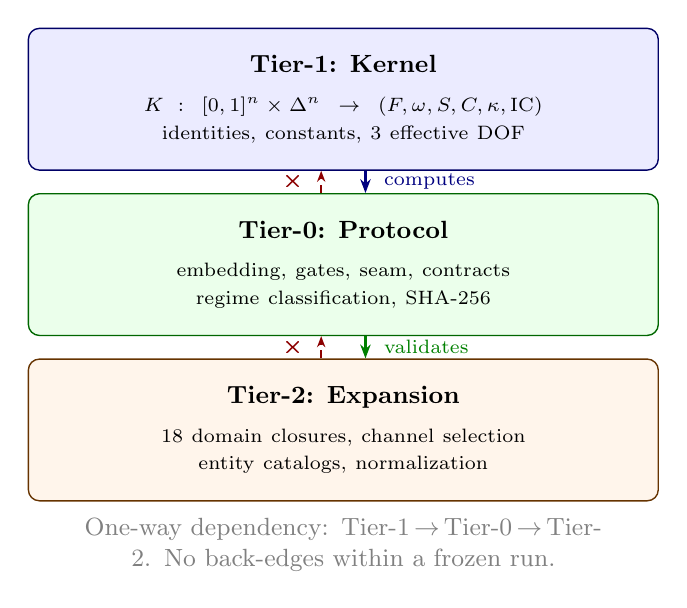
\begin{tikzpicture}[
  tier/.style={
    draw, thick, rounded corners=4pt,
    minimum width=8.0cm, minimum height=1.8cm,
    text width=7.4cm, align=center,
    font=\small, line width=0.5pt
  },
  fwd/.style={-{Stealth[length=5pt]}, line width=0.8pt},
  back/.style={-{Stealth[length=4pt]}, line width=0.6pt,
    red!55!black, densely dashed}]

% Tier boxes — full column width, generous spacing
\node[tier, fill=blue!8, draw=blue!40!black] (t1) at (0,4.2)
  {\textbf{Tier-1: Kernel}\\[3pt]
   {\scriptsize $K\!: [0,1]^n\!\times\!\Delta^n
     \to (F,\omega,S,C,\kappa,\IC)$}\\[-1pt]
   {\scriptsize identities, constants, 3 effective DOF}};

\node[tier, fill=green!8, draw=green!40!black] (t0) at (0,2.1)
  {\textbf{Tier-0: Protocol}\\[3pt]
   {\scriptsize embedding, gates, seam, contracts}\\[-1pt]
   {\scriptsize regime classification, SHA-256}};

\node[tier, fill=orange!8, draw=orange!40!black] (t2) at (0,0)
  {\textbf{Tier-2: Expansion}\\[3pt]
   {\scriptsize 18 domain closures, channel selection}\\[-1pt]
   {\scriptsize entity catalogs, normalization}};

% Forward arrows (right side) — dependency flows downward
\draw[fwd, blue!50!black]
  ([xshift=8pt]t1.south) -- ([xshift=8pt]t0.north)
  node[midway, right=3pt, font=\scriptsize] {computes};
\draw[fwd, green!50!black]
  ([xshift=8pt]t0.south) -- ([xshift=8pt]t2.north)
  node[midway, right=3pt, font=\scriptsize] {validates};

% Forbidden back-edges (left side) — with prohibition marks
\draw[back]
  ([xshift=-8pt]t2.north) -- ([xshift=-8pt]t0.south)
  node[midway, font=\bfseries\scriptsize,
    text=red!55!black, left=3pt] {\texttimes};
\draw[back]
  ([xshift=-8pt]t0.north) -- ([xshift=-8pt]t1.south)
  node[midway, font=\bfseries\scriptsize,
    text=red!55!black, left=3pt] {\texttimes};

% Immutability annotation
\node[font=\small, text=black!50,
  anchor=north, text width=7.4cm, align=center]
  at (0, -1.0)
  {One-way dependency: Tier-1\,$\to$\,Tier-0\,$\to$\,Tier-2.
   No back-edges within a frozen run.};

\end{tikzpicture}
\caption{Three-tier architecture.  Dependency flows
downward: the kernel function (Tier-1) is computed by
protocol code (Tier-0), which validates domain closures
(Tier-2).  Dashed red arrows with \texttimes\ marks
indicate forbidden back-edges: no Tier-2 output may modify
Tier-0 or Tier-1 within a frozen run.  Promotion from
Tier-2 to Tier-1 requires a formal seam weld.}
\label{fig:tiers}
\end{figure*}

% -------------------------------------------------------------
% Figure: Regime Partition (placed after Tiers for layout)
% -------------------------------------------------------------
\begin{figure*}[t!]
\centering
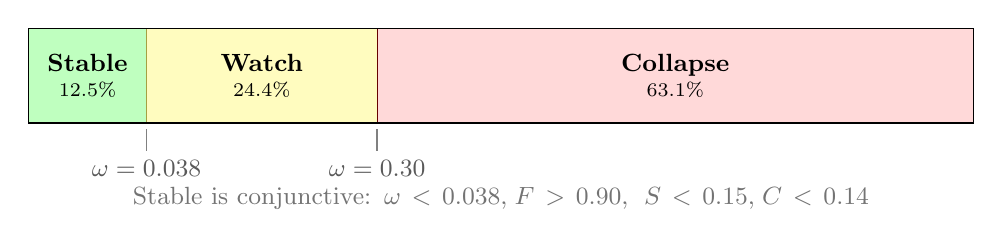
\begin{tikzpicture}
  % Horizontal stacked bar — full width
  \def\totalw{12.0}
  \def\barh{1.2}

  % Filled regions proportional to Fisher-space volume
  \fill[green!25, draw=green!50!black, line width=0.4pt]
    (0,0) rectangle (1.5,\barh);
  \fill[yellow!25, draw=yellow!60!black, line width=0.4pt]
    (1.5,0) rectangle (4.428,\barh);
  \fill[red!15, draw=red!40!black, line width=0.4pt]
    (4.428,0) rectangle (\totalw,\barh);

  % Outer frame
  \draw[line width=0.6pt] (0,0) rectangle (\totalw,\barh);

  % Labels inside each segment
  \node[font=\small, align=center]
    at (0.75, 0.6) {\textbf{Stable}\\[-2pt]
    {\scriptsize 12.5\%}};
  \node[font=\small, align=center]
    at (2.964, 0.6) {\textbf{Watch}\\[-2pt]
    {\scriptsize 24.4\%}};
  \node[font=\small, align=center]
    at (8.214, 0.6) {\textbf{Collapse}\\[-2pt]
    {\scriptsize 63.1\%}};

  % Threshold markers with tick lines below
  \draw[line width=0.5pt, black!50]
    (1.5, -0.08) -- (1.5, -0.35);
  \draw[line width=0.5pt, black!50]
    (4.428, -0.08) -- (4.428, -0.35);
  \node[font=\small, text=black!65, below]
    at (1.5, -0.35) {$\omega = 0.038$};
  \node[font=\small, text=black!65, below]
    at (4.428, -0.35) {$\omega = 0.30$};

  % Gate annotation — compact, below
  \node[font=\small, text=black!55,
    text width=10cm, align=center]
    at (6.0, -0.95)
    {Stable is conjunctive: $\omega < 0.038$,\;$F > 0.90$,
     \;$S < 0.15$,\;$C < 0.14$};
\end{tikzpicture}
\caption{Regime partition of the Bernoulli manifold in
Fisher space~\cite{fisher1925,amari2016information}, with
bar widths proportional to volume.  Stable occupies only
12.5\% of the manifold; Watch 24.4\%; Collapse 63.1\%.
Stability is rare---87.5\% of the manifold lies outside
it.  The Stable regime is conjunctive: all four gates must
be satisfied simultaneously.}
\label{fig:regimes}
\end{figure*}

% -------------------------------------------------------------
% Figure: The Discourse Spine
% -------------------------------------------------------------
\begin{figure*}[t!]
\centering
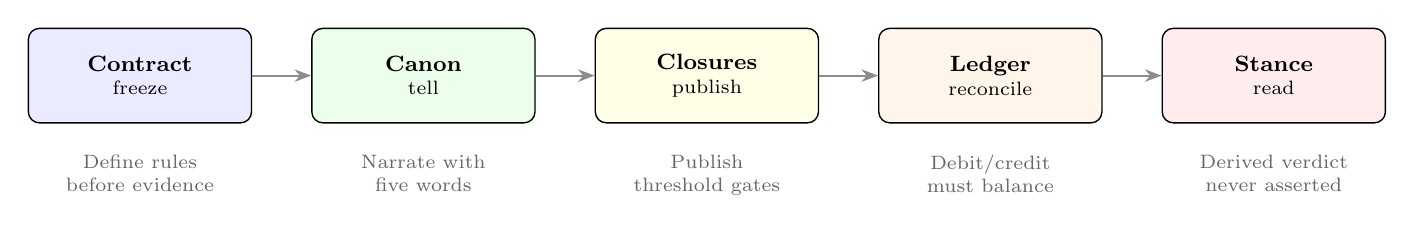
\begin{tikzpicture}[
  box/.style={
    draw, thick, rounded corners=4pt,
    minimum width=2.8cm, minimum height=1.2cm,
    text width=2.6cm, align=center,
    font=\footnotesize, fill=#1, line width=0.5pt
  },
  arr/.style={-{Stealth[length=6pt]}, line width=0.8pt,
    black!45},
  ann/.style={font=\scriptsize, text=black!60,
    text width=2.6cm, align=center}]

% Five stops — evenly spaced
\node[box=blue!8]    (c) at (0,0)
  {\textbf{Contract}\\[-1pt]{\scriptsize freeze}};
\node[box=green!8]   (n) at (3.6,0)
  {\textbf{Canon}\\[-1pt]{\scriptsize tell}};
\node[box=yellow!10] (l) at (7.2,0)
  {\textbf{Closures}\\[-1pt]{\scriptsize publish}};
\node[box=orange!8]  (g) at (10.8,0)
  {\textbf{Ledger}\\[-1pt]{\scriptsize reconcile}};
\node[box=red!7]     (s) at (14.4,0)
  {\textbf{Stance}\\[-1pt]{\scriptsize read}};

% Connecting arrows
\draw[arr] (c) -- (n);
\draw[arr] (n) -- (l);
\draw[arr] (l) -- (g);
\draw[arr] (g) -- (s);

% Annotations below each box — all same font
\node[ann, below=8pt] at (c.south)
  {Define rules\\before evidence};
\node[ann, below=8pt] at (n.south)
  {Narrate with\\five words};
\node[ann, below=8pt] at (l.south)
  {Publish\\threshold gates};
\node[ann, below=8pt] at (g.south)
  {Debit/credit\\must balance};
\node[ann, below=8pt] at (s.south)
  {Derived verdict\\never asserted};

\end{tikzpicture}
\caption{The discourse spine: every claim follows five
mandatory stops, in order.  The Contract freezes rules
before evidence.  The Canon narrates using five words
(Drift, Fidelity, Roughness, Return, Integrity).
Closures publish threshold gates.  The Integrity Ledger
debits Drift and Roughness, credits Return; the residual
must close ($\leq \tolseam$).  The Stance is the derived
verdict (Stable/Watch/Collapse), never asserted.  Removing
any stop removes a provable guarantee.}
\label{fig:spine}
\end{figure*}

% -------------------------------------------------------------
% Figure 4: Geometric Slaughter
% -------------------------------------------------------------
\begin{figure*}[t!]
\centering
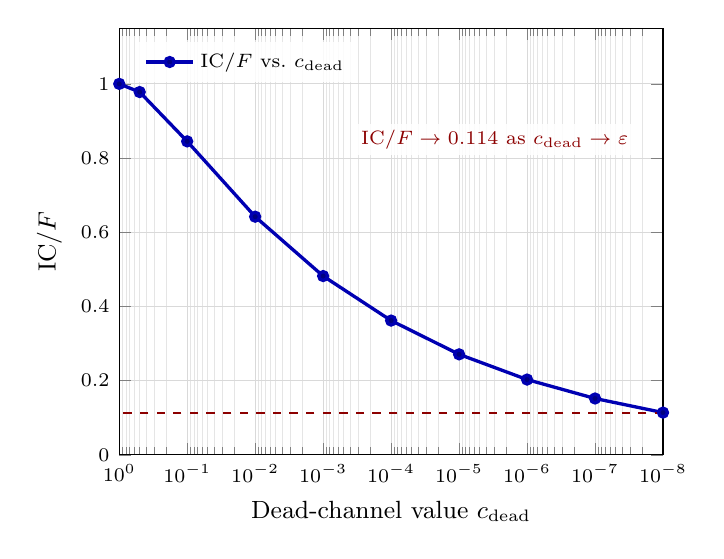
\begin{tikzpicture}
\begin{axis}[
  width=0.7\textwidth,
  height=7cm,
  xmode=log,
  xlabel={Dead-channel value $c_\mathrm{dead}$},
  ylabel={$\IC/F$},
  xmin=1e-8, xmax=1,
  ymin=0, ymax=1.15,
  grid=both,
  grid style={gray!20, line width=0.2pt},
  major grid style={gray!30, line width=0.3pt},
  tick label style={font=\scriptsize},
  label style={font=\small},
  x dir=reverse,
  every axis plot/.append style={line width=1.2pt},
  legend style={font=\scriptsize, at={(0.03,0.97)},
    anchor=north west, draw=none, fill=white, fill opacity=0.85,
    text opacity=1}]

% Main curve
\addplot[blue!70!black, mark=*, mark size=1.6pt,
  mark options={fill=blue!50!black}]
  coordinates {
  (0.999, 1.000)
  (0.5,   0.978)
  (0.1,   0.845)
  (0.01,  0.642)
  (1e-3,  0.482)
  (1e-4,  0.362)
  (1e-5,  0.271)
  (1e-6,  0.203)
  (1e-7,  0.152)
  (1e-8,  0.114)
};
\addlegendentry{$\IC/F$ vs.\ $c_\mathrm{dead}$}

% Asymptotic floor — dashed reference line
\addplot[dashed, red!55!black, line width=0.7pt,
  forget plot]
  coordinates {(1e-8, 0.114) (0.999, 0.114)};
\addlegendentry{floor at $\eps = 10^{-8}$}

% Floor value label — in open space, upper left
\node[font=\scriptsize, text=red!55!black,
  fill=white, fill opacity=0.85, text opacity=1,
  inner sep=2pt]
  at (axis cs:3e-6, 0.85)
  {$\IC/F \to 0.114$ as $c_\mathrm{dead} \to \eps$};

\end{axis}
\end{tikzpicture}
\caption{Geometric slaughter: one dead channel destroys
multiplicative coherence.  An 8-channel trace with
7~channels at $c = 0.999$ and 1~channel at
$c_\mathrm{dead}$.  As the dead channel approaches
$\eps = 10^{-8}$, $\IC/F$ drops to $\approx 0.114$
while $F$ remains healthy at $0.874$.  This mechanism
underlies confinement detection~\cite{wilson1974confinement}
in the Standard Model closure~\cite{pdg2024}: the color
channel at $c \approx \eps$ in hadrons produces
$\IC/F < 0.04$, making the quark${\to}$hadron boundary
visible as a $100{\times}$ drop.}
\label{fig:slaughter}
\end{figure*}

% -------------------------------------------------------------
% Figure 5: Equator Structure
% -------------------------------------------------------------
\begin{figure*}[t!]
\centering
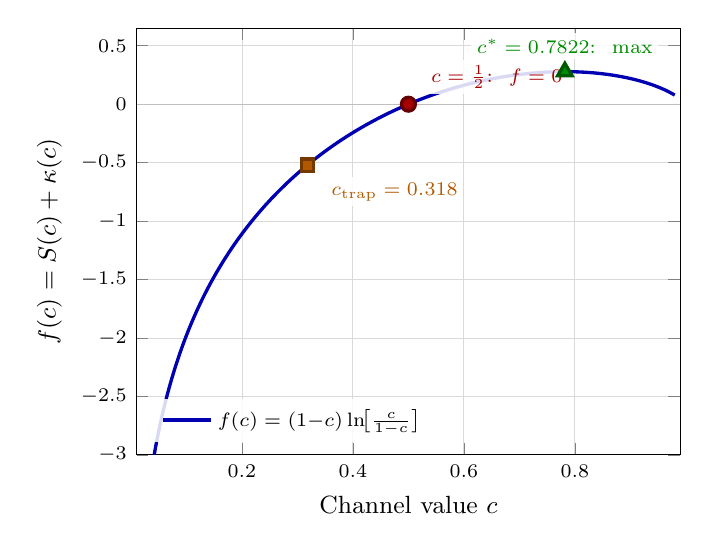
\begin{tikzpicture}
\begin{axis}[
  width=0.7\textwidth,
  height=7cm,
  xlabel={Channel value $c$},
  ylabel={$f(c) = S(c) + \kappa(c)$},
  xmin=0.01, xmax=0.99,
  ymin=-3.0, ymax=0.65,
  grid=both,
  grid style={gray!20, line width=0.2pt},
  major grid style={gray!30, line width=0.3pt},
  tick label style={font=\scriptsize},
  label style={font=\small},
  ytick={-3,-2.5,-2,-1.5,-1,-0.5,0,0.5},
  every axis plot/.append style={line width=1.2pt},
  legend style={font=\scriptsize, at={(0.03,0.03)},
    anchor=south west, draw=none, fill=white,
    fill opacity=0.85, text opacity=1}]

% Main curve with dense sampling
\addplot[blue!70!black, smooth, samples=80,
  domain=0.02:0.98]
  {(1-x)*ln(x/(1-x))};
\addlegendentry{$f(c) = (1{-}c)\ln\!\bigl[\frac{c}{1-c}\bigr]$}

% Zero line for reference
\draw[black!25, line width=0.4pt]
  (axis cs:0.01, 0) -- (axis cs:0.99, 0);

% Equator: c = 1/2 — zero crossing
\addplot[only marks, mark=*, mark size=2.5pt,
  mark options={fill=red!65!black, draw=red!40!black},
  forget plot]
  coordinates {(0.50, 0.0)};
\node[font=\scriptsize, text=red!65!black,
  fill=white, fill opacity=0.85, text opacity=1,
  inner sep=2pt, anchor=south west]
  at (axis cs:0.53, 0.08)
  {$c = \tfrac{1}{2}$:\; $f = 0$};

% Maximum: c* = 0.782
\addplot[only marks, mark=triangle*, mark size=3pt,
  mark options={fill=green!55!black, draw=green!35!black},
  forget plot]
  coordinates {(0.782, 0.279)};
\node[font=\scriptsize, text=green!55!black,
  fill=white, fill opacity=0.85, text opacity=1,
  inner sep=2pt, anchor=south]
  at (axis cs:0.782, 0.38)
  {$c^* = 0.7822$:\; max};

% Cardano root: c_trap = 0.318
\addplot[only marks, mark=square*, mark size=2.2pt,
  mark options={fill=orange!70!black, draw=orange!45!black},
  forget plot]
  coordinates {(0.318, -0.521)};
\node[font=\scriptsize, text=orange!70!black,
  fill=white, fill opacity=0.85, text opacity=1,
  inner sep=2pt, anchor=north west]
  at (axis cs:0.35, -0.62)
  {$c_\mathrm{trap} = 0.318$};

\end{axis}
\end{tikzpicture}
\caption{The function
$f(c) = S(c) + \kappa(c)$ on a
single Bernoulli channel, verified to $< 10^{-16}$ against
the closed form $f(c) = (1{-}c)\ln[c/(1{-}c)]$.  Three
structural landmarks: the \emph{equator} $c = \tfrac{1}{2}$
where $f = 0$ exactly (quintuple fixed point); the
\emph{logistic self-dual} point $c^* = 0.7822$ where $f$
reaches its global maximum; and the \emph{Cardano root}
$c_\mathrm{trap} = 0.3178$ of $x^3 + x - 1 = 0$ where
$\Gam$ first drops below~1.  These three points form the
skeleton of the Bernoulli manifold.}
\label{fig:equator}
\end{figure*}

% -------------------------------------------------------------
% Figure 6: Solvability Region
% -------------------------------------------------------------
\begin{figure*}[t!]
\centering
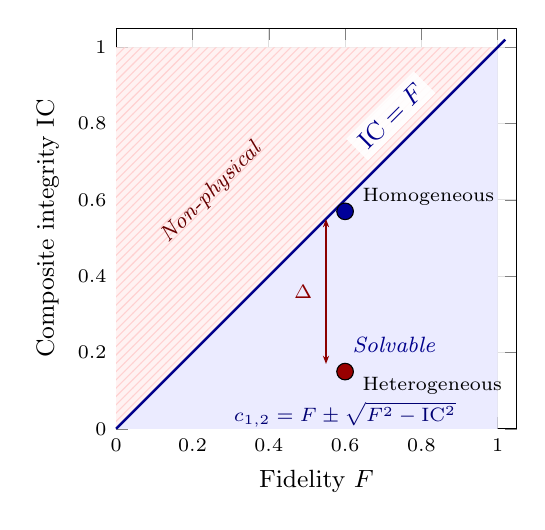
\begin{tikzpicture}
\begin{axis}[
  width=0.55\textwidth,
  height=0.55\textwidth,
  xlabel={Fidelity $F$},
  ylabel={Composite integrity $\IC$},
  xmin=0, xmax=1.05,
  ymin=0, ymax=1.05,
  xtick={0, 0.2, 0.4, 0.6, 0.8, 1.0},
  ytick={0, 0.2, 0.4, 0.6, 0.8, 1.0},
  tick label style={font=\scriptsize},
  label style={font=\small},
  grid=both,
  grid style={gray!15, line width=0.2pt},
  major grid style={gray!25, line width=0.3pt},
  axis equal image,
  clip=false]

% Solvable region — below diagonal
\addplot[fill=blue!8, draw=none, forget plot]
  coordinates {(0,0) (1,1) (1,0)} \closedcycle;

% Non-physical region — above diagonal (hatched)
\addplot[fill=red!5, draw=none,
  postaction={pattern=north east lines,
    pattern color=red!18}, forget plot]
  coordinates {(0,0) (1,1) (0,1)} \closedcycle;

% Diagonal: IC = F
\addplot[blue!55!black, thick, line width=0.9pt,
  forget plot]
  coordinates {(0,0) (1.02,1.02)};

% Diagonal label — clearly above the line
\node[font=\small, text=blue!55!black, rotate=45,
  fill=white, fill opacity=0.9, text opacity=1,
  inner sep=2.5pt]
  at (axis cs:0.72, 0.82)
  {$\IC = F$};

% Region labels
\node[font=\footnotesize, text=blue!55!black]
  at (axis cs:0.73, 0.22) {\textit{Solvable}};
\node[font=\footnotesize, text=red!40!black, rotate=45]
  at (axis cs:0.25, 0.62) {\textit{Non-physical}};

% Example points — homogeneous (near diagonal)
\addplot[only marks, mark=*, mark size=3pt,
  mark options={fill=blue!60!black}, forget plot]
  coordinates {(0.60, 0.57)};
\node[font=\scriptsize, anchor=south west, inner sep=2pt]
  at (axis cs:0.63, 0.57) {Homogeneous};

% Example points — heterogeneous (far from diagonal)
\addplot[only marks, mark=*, mark size=3pt,
  mark options={fill=red!60!black}, forget plot]
  coordinates {(0.60, 0.15)};
\node[font=\scriptsize, anchor=north west, inner sep=2pt]
  at (axis cs:0.63, 0.15) {Heterogeneous};

% Gap annotation
\draw[{Stealth[length=3pt]}-{Stealth[length=3pt]},
  red!55!black, line width=0.6pt]
  (axis cs:0.55, 0.17) -- (axis cs:0.55, 0.55);
\node[font=\scriptsize, text=red!55!black,
  anchor=east, inner sep=2pt]
  at (axis cs:0.53, 0.36) {$\Delta$};

% Recovery formula — bottom right, clear space
\node[font=\scriptsize, text=blue!45!black,
  anchor=north west, inner sep=1pt]
  at (axis cs:0.30, 0.08)
  {$c_{1,2} = F \pm \sqrt{F^2 - \IC^2}$};

\end{axis}
\end{tikzpicture}
\caption{Solvability region in the $(F, \IC)$
plane for a rank-2 trace.  Below the
diagonal $\IC = F$, individual channel values
$c_{1,2} = F \pm \sqrt{F^2 - \IC^2}$ are real---the trace
is physically realizable.  Above the diagonal, no trace
exists with those aggregate invariants.  The heterogeneity
gap $\Delta = F - \IC$ measures deviation from the diagonal.
The integrity bound $\IC \leq F$ is a \emph{solvability
condition}---it guarantees that the kernel's inverse problem
has real solutions---not merely an algebraic inequality.}
\label{fig:solvability}
\end{figure*}

\clearpage
\twocolumngrid
\bibliography{Bibliography}

\end{document}
